\documentclass[a4paper,11pt]{report}
\pdfoutput=1 % if your are submitting a pdflatex (i.e. if you have
             % images in pdf, png or jpg format)

\usepackage{jheppub} % for details on the use of the package, please
                     % see the JHEP-author-manual

\usepackage[T1]{fontenc} % if needed

%**************** Utilities **************
\usepackage{lipsum}
\usepackage{comment}
\usepackage{enumitem}
\usepackage{color}

% *************** Math and Physics *************
\usepackage{mathtools} % per valore assoluto e norma
\usepackage{braket} % per i comandi \Set e \Bra e simili
\usepackage{amsthm} % per teoremi e dimostrazioni
\usepackage{tensor} % per tensori e indici alto/basso
\usepackage{physics}
\usepackage{braket}
\usepackage{dsfont}
% ******************************************
% ******************************************************************************
% *************************** INSIEMISTICA *************************************
\newcommand{\numberset}{\mathbb}
\newcommand{\N}{\numberset{N}}
\newcommand{\Z}{\numberset{Z}}
\newcommand{\R}{\numberset{R}}
\newcommand{\C}{\numberset{C}}
\newcommand{\1}{\mathds{1}}
% ******************************************************************************
% ****************************** OPERATORS **************************************
%\DeclarePairedDelimiter{\abs}{\lvert}{\rvert}
\DeclarePairedDelimiter{\mynorm}{\lVert}{\rVert}
\DeclarePairedDelimiter{\inner}{\langle}{\rangle}
\DeclareMathOperator{\sgn}{sgn}
\DeclareMathOperator{\Realpart}{Re} % ridefinisco parte reale
\DeclareMathOperator{\Impart}{Im}
\renewcommand{\Re}{\Realpart} % ridefinisco parte reale (altrimenti dà simbolo in gotico)
\renewcommand{\Im}{\Impart} 
\DeclareMathOperator*{\argmax}{arg\,max}
%\DeclareMathOperator{\Tr}{Tr}
%\DeclareMathOperator{\Res}{Res}


% ******************************************************************************
% *************************** VECTOR CALCULUS **********************************
\newcommand{\bcdot}{\boldsymbol{\cdot}} % così \bcdot è prodotto scalare in grassetto
\renewcommand{\vec}{\boldsymbol}
\newcommand{\del}{\vec{\nabla}}


% ******************************************************************************
% *************************** DIFFERENTIATION **********************************
\newcommand{\ud}{\mathop{}\!\mathrm{d}}
\newcommand{\udd}{{\ud}^2}
\newcommand{\udt}{{\ud}^3}
\newcommand{\udq}{{\ud}^4}
\newcommand{\bb}[1]{\mathbb{#1}}
\newcommand{\de}{\partial}


% ******************************************************************************
% ******************************* THEOREMS *************************************
\theoremstyle{plain}
\newtheorem{theorem}{Theorem}

\theoremstyle{plain}
\newtheorem*{principle}{Principle}

\theoremstyle{plain}
\newtheorem{lemma}{Lemma}

\theoremstyle{definition}
\newtheorem{definition}{Definition}

\theoremstyle{remark}
\newtheorem*{remark}{Remark}

\renewcommand{\thelemma}{L.\arabic{lemma}}
\renewcommand{\thetheorem}{T.\arabic{theorem}}

\newenvironment{innerproof}
 {\renewcommand{\qedsymbol}{}\proof}
 {\endproof}

% ******************************************************************************
% ******************************* SHORTCUTS ************************************
\newcommand{\invgamma}{\sqrt{1- \frac{v^2}{c^2}}}
\renewcommand{\L}{\mathcal{L}}
\newcommand{\g}{\mathfrak{g}}
\newcommand{\h}{\mathfrak{h}}
\newcommand{\M}{\mathcal{M}}
\newcommand{\D}{\mathcal{D}}
\newcommand{\qi}{q^{(m)}}
\newcommand{\qf}{q^{(g)}}
\newcommand{\bdelta}{\bar{\delta}}
\newcommand{\deltat}{{\delta}^3}
\newcommand{\deltaq}{{\delta}^4}
\renewcommand{\epsilon}{\varepsilon}
\newcommand{\phis}{{\phi}^*}
\newcommand{\hbarq}{{\hbar}^2}
\renewcommand{\H}{\mathcal{H}}
\newcommand{\q}{\hat{\vec{q}}}
\newcommand{\Tau}{\mathcal{T}}
\newcommand{\ray}{\mathcal{R}}

% ******************************************************************************
% ************************ SHORTCUTS WITH ARGUMENTS ****************************
\newcommand{\bravec}[1]{\bra{\vec{#1}}} 
\newcommand{\ketvec}[1]{\ket{\vec{#1}}} 
\renewcommand{\op}[1]{\hat{#1}}
\newcommand{\opvec}[1]{\op{\vec{#1}}}
\newcommand{\dual}[1]{\widetilde{#1}}
\DeclareMathOperator{\Aut}{Aut}
\DeclareMathOperator{\id}{id}

% ******************************************************************************
% ******************************** GRAPHICS ************************************
\renewcommand\qedsymbol{$\blacksquare$}

% ******************************************************************************
% ******************************** matrices and scalar prodict ************************
\newcommand{\irow}[1]{% inline row vector
  \begin{smallmatrix}(\,#1\,)\end{smallmatrix}%
}

\newcommand{\icol}[1]{% inline column vector
  \left(\begin{smallmatrix}#1\end{smallmatrix}\right)%
}

\newcommand{\scalar}[2]{\langle #1, #2 \rangle}
\renewcommand{\norm}[1]{\scalar{#1}{#1}}
\newcommand{\tev}{\textup{TeV}}

% **************** PROOF BACKGROUND *************
\usepackage[dvipsnames]{xcolor}
\usepackage{mdframed}
\mdfsetup{%
linecolor=black,
backgroundcolor=gray!6,
}

\usepackage{bm}
\usepackage{array}
\usepackage{multirow}
\renewcommand{\arraystretch}{1.3}


%%%%%%%%%%%%%%%%%%% JHEP SETTINGS %%%%%%%%%%%%%%%%%%%%%%%

\bibliographystyle{jhep}

\title{Circle Compactifications}

\author[a]{Giancarlo Oancia}
\affiliation[a]{University of Bologna}

\emailAdd{giancarlo.oancia@studio.unibo.it} 


\abstract{This document discusses the compactification of strings on circles, and how type IIA and IIB are related by T-duality. This is \emph{not} an original work, and its purpose is to prepare the string theory exam of UNIBO. We follow the conventions of the university lectures by professor Ling Lin~\cite{ling:strings}, while the development mostly follows~\cite{uranga:strings}. Other references used are~\cite{polchisnki:strings, polchisnki:superstrings, ibanez:strings, grana:strings, weigand:strings, blum:basic}.}

\keywords{Strings, Compactification, T-duality}

%%%%%%%%%%%%%%%% CHAPTER GRAPHICS %%%%%%%%%%%%
\usepackage{titlesec}
\titleformat{\chapter}{}{}{0em}{\bf\LARGE}



%%%%%%%%%%%%%%%% DOCUMENT %%%%%%%%%%%%%%%%%%%%%%%%
\begin{document}
\maketitle
\flushbottom
\addtocontents{toc}{\protect\thispagestyle{empty}}

\chapter{Kaluza-Klein Compactification in Field Theory}
\pagenumbering{arabic}
Consider a field theory in $D$ dimensions propagating in a background spacetime of the form $\M_D = \M_d \times S^1$, where $D = d+1$. Let's call $x^{\hat{\mu}} = (x^\mu, y)$ the coordinates in $\M_D$, where $\hat{\mu} = 0, \dots, D-1 = d$, $\mu = 0, \dots, d-1$ and on the internal space $S^1$ we identify $y \simeq y = 2\pi R$.

%***************** KK REDUCTION OF SCALAR FIELD ********************
\section{KK Reduction of a Scalar Field on \texorpdfstring{$S^1$}{S1}}
The masses of the Kaluza-Klein modes are integer multiples of the compactification scale $M_c = 1 / R$, so, we can ignore them in the limit
    \begin{equation}
        E \ll M_c = 1/R
    \end{equation}


%***************** KK REDUCTION OF GRAVITY ********************
\section{KK Reduction of Einstein Theory on \texorpdfstring{$S^1$}{S1}}
In particular, consider a $D$-dimensional Einstein theory, with metric $G_{\hat{\mu} \hat{\nu}} (x^{\hat{\mu}})$.

Exploiting the periodicity in the internal space, we may expand the metric in Fourier modes as
\begin{equation}
    G_{\hat{\mu} \hat{\nu}} (x^{\hat{\mu}}) = G_{\hat{\mu} \hat{\nu}} (x^\mu, y) = G^{(0)}_{\hat{\mu} \hat{\nu}} (x^\mu)+ \sum_{s \neq 0} G^{(s)}_{\hat{\mu} \hat{\nu}} (x^\mu) e^{i s y / R}.
\end{equation}

However, we're interested in the $(D-1)$-dimensional theory, so it's more convenient to first decompose $SO(1,D-1)$'s representations into representations of $SO(1,d-1)$. After the decomposition, we can exploit the periodicity of the internal space and Fourier expand as usual. In particular, recalling that we defined $x^{D-1} = x^d = y$, the graviton decomposes as
\begin{align}
    G_{\hat{\mu}\hat{\nu}} (x^\mu, y) 
    &\to G_{\mu\nu}(x^\mu, y) = G^{(0)}_{{\mu} {\nu}} (x^\mu)+ \sum_{s \neq 0} G^{(s)}_{{\mu} {\nu}} (x^\mu) e^{is y / R} ,\\
    &\to G_{\mu d} (x^\mu, y) = G^{(0)}_{{\mu} {d}} (x^\mu)+ \sum_{s \neq 0} G^{(s)}_{{\mu} {d}} (x^\mu) e^{is y / R} ,\\
    &\to G_{dd} (x^\mu, y) = G^{(0)}_{{d} {d}} (x^\mu)+ \sum_{s \neq 0} G^{(s)}_{{d} {d}} (x^\mu) e^{is y / R} . \\
\end{align}

It's straightforward to observe that the massless modes are a $d$-dimensional graviton, a $d$-dimensional scalar and a $d$-dimensional $U(1)$ gauge boson. To be more precise, if we call the zero-modes fields $g_{\mu\nu}(x^\mu), A_\mu(x^\mu), \phi(x^\mu)$, then, they're related to the zero-mode five-dimensional metric by
\begin{equation}
    G^{(0)}_{\hat{\mu}\hat{\nu}} = 
    \begin{pmatrix}
        e^{2\alpha_d} g_{\mu\nu} + e^{-2(d-2)\alpha_d \phi} A_\mu A_\nu & e^{-2(d-2)\alpha_d \phi} A_\mu \\
        e^{-2(d-2)\alpha_d \phi} A_\nu & e^{-2(d-2)\alpha_d \phi}
    \end{pmatrix} ,
\end{equation}
where we defined $\alpha_d$ in such a way that the action in dimension $D-1 = d$ is canonically normalized. In particular,
\begin{equation}
    \alpha_d = \sqrt{\frac{1}{2(d-1)(d-2)}} .
\end{equation}

From a zero-mode Kaluza-Klein point of view, this leads to the metric
\begin{equation}\label{eq:kk-metric-decomp}
    \ud s^2 = G^{(0)}_{\hat{\mu}\hat{\nu}} \ud x^{\hat{\mu}} \ud x^{\hat{\nu}} + \dots = e^{2\alpha_d \phi} g_{\mu\nu} \ud x^\mu \ud x^\nu + e^{-2(d-2)\alpha_d \phi} (\ud y + A_\mu \ud x^\mu)^2 + \dots.
\end{equation}
In particular, it allows for $d$-dimensional reparametrizations $x'^\mu(x^\nu)$ and for reparametrizations of the internal space coordinates $y' = y + \lambda(x^\mu)$. To make the theory invariant under the latter transformations, the field $A_\mu$ must transform under the $U(1)$ transformation $A'_\mu = A_\mu - \de_\mu \lambda$, which is straightforward, looking at~\eqref{eq:kk-metric-decomp}.

Therefore, we observe that the gauge transformations of the vector boson follow from coordinate reparametrization in the internal dimension. At the end, gauge invariance after dimensional reduction follows from diffeomorphism invariance in higher dimensions. Baiscally, under the compactification ansatz $\M_D \to \M_d \times S^1$, the group of diffeomorphisms decomposes as
\begin{equation}
    Gl(D, \R) \to Gl(d,\R) \times U(1).
\end{equation}

This was the original motivation of Kaluza-Klein, to unify gravity with gauge theories. However, this way we can't obtain charges chiral fermions, so this attempt failed.

Another interesting feature of Kaluza-Klein compactifications is the arising of \emph{moduli}, which are massless scalar fields in $d$-dimensions with no potential. In this example, this is acheved by the field $\phi$, called \emph{radion}. It sets the volume of the internal space, since
\begin{equation}
    \textup{Vol} (S^1)  = \int_{0}^{2\pi R} \ud^d x \sqrt{G_{dd}} \cdot 2\pi R = e^{-2(d-2)\alpha_d \phi} \cdot 2\pi R .
\end{equation}

To observe that it isn't constraint by a potential, let's fix the ideas and consider the case $D=5$, $d=4$. The theory is represented by the action
\begin{equation}
    S_5 = \frac{M^3_5}{2} \int \ud^5 x \sqrt{-G} R_5,
\end{equation}
where $G_5 = \det(G_{\hat{\mu} \hat{\nu}})$, and $R_5$ is the Ricci scalar. Substituting the above metric for the zero-modes, after working out the Ricci scalar, we get a $4$ dimensional action which reads
\begin{equation}
    S_4 = M^3_5 \pi R \int \udq x \sqrt{-g} \left( R_4 -\frac{1}{6} \de_\mu \phi \de^\mu \phi - \frac{1}{4 e^\phi} F_{\mu\nu} F^{\mu\nu} + \textup{KK tower \dots} \right),
\end{equation}
where the constant is compatible with the $4d$ gravity action
\begin{equation}
    S_4 = \frac{M^2_p}{16\pi} \int \udq x \sqrt{-g} R_4 ,
\end{equation}
if
\begin{equation}\label{eq:relation-plank-masses}
    M^2_p = 16 \pi^2 M^3_5 R,
\end{equation}
and gauge coupling $g^2 = e^\phi$. The above relation~\eqref{eq:relation-plank-masses} suggests us that there's the possibility to have a low fundamental gravity scale $M_5$, if we take $R$ large enough. However, following the idea of Kaluza-Klein, this approach fails if we try to couple with the standard model, since we know that the KK-masses are proportional to the scale $M_c = 1/R$, so, for large $R$ we'd get too light KK modes, which should've been observed. This leads to the idea of a \emph{brane-world scenario}.

\paragraph{Brane-World scenario}
Even if in the first years people focused on type I string theories since they contain gauge theories, there had been a revival of type II theories after the discovery of branes. In particular, the idea is that \emph{closed strings}, which contains the graviton, propagates on the bulk of the theory, which is $10$-dimensional for the superstring. Further, open strings are attached to branes, which are submanifolds of the bulk on which Standard Model fields live in, considering that stack of branes could lead to non-abelian gauge theories. 

One simple example is considering the standard model fields localized on a $3$-brane, which exists for a type IIB theory (double check it), so that the action splits into a $4$ dimensional piece for the $3$-brane worldvolume, and a bulk piece in the larger $10$-dimensional spacetime
\begin{equation}
    S_\textup{brane-world} = S_\textup{brane} + S_\textup{bulk} = \int \udq x \L_\textup{brane} + \int d^{10} x \L_\textup{bulk} .
\end{equation}
Then, gravity is compactified as discussed earlier, while gauge and matter fields are insensitive of the compactification procedure, and then they don't have massive KK modes. This allows for \emph{large extra dimensions}, whose size is in principle detectable only through the effect on gravity. Looking again at~\eqref{eq:relation-plank-masses}, we can even have $M_5 \simeq \tev$, so that there would be no hierarchy between the EW and the gravitational scale. However, this is not a fully satisfactory resolution, since we've moved the problem into a hierarchy problem between the large size $1/R$ of the extra dimension, and the fundamental scale $1/M_5$. Another possibility is provided by the \emph{Randall-Sundrum Scenario}

\paragraph{Randall-Sundrum Scenario}
Still to be written, look at Quevedo and Ibanez.

\chapter{Closed Bosonic String}
%******************** MODE EXPANSION *********************
\section{Mode Expansion}
We use mostly plus metric $\eta = \textup{diag}(-,+,\dots,+)$ and focus on \emph{closed strings}. We already focus on the \emph{critical string}, considering as a background the flat $26d$ Minkowski spacetime $\M_{26}$.

The worldsheet coordinates are $\xi^a = (\tau, \sigma)$, $a= 1,2$, where $\sigma \in (0,l)$. Taking as a background the flat $26$-dimensional Minkowski spacetime $\M_{26}$, the string is described by the worldsheet fields $X^{{\mu}}$, with ${\mu} = 0, \dots, 25$. Considering the $2d$ metric $\gamma_{ab}(\xi^a)$, the Polyakov action reads
\begin{equation}
    S_P= -\frac{1}{4\pi\alpha'} \int_\Sigma \ud^2 \xi \sqrt{-\gamma} \, \gamma^{ab} \de_a X^{{\mu}} \de_b X^{{\nu}} \eta_{{\mu}{\nu}} ,
\end{equation}
where the string tension is
\begin{equation}
    T = \frac{1}{2\pi\alpha'} .
\end{equation}

Exploiting the reparametrisation invariance and the Weyl symmetry, we can go to \emph{conformal gauge}, in which $\gamma_{ab} = \eta_{ab}$, such that Polyakov action becomes
\begin{equation}\label{eq:polyakov-conformal-gauge}
    S_P= -\frac{1}{4\pi\alpha'} \int_\Sigma \ud^2 \xi \, \de_a X^{{\mu}} \de^a X_{{\nu}}  .
\end{equation}

Defining \emph{worldsheet lightcone coordinates} $\xi^\pm \equiv \tau \pm \sigma$, the equations of motion read $\de_+\de_- X^\mu = 0$, which is solved by the ansatz
\begin{equation}\label{eq:left-right-movers-def}
    X^{{\mu}}(\xi^a) = X^{{\mu}}_L(\xi^+) + X^{{\mu}}_R(\xi^-) ,
\end{equation}
where $\xi^\pm \equiv \tau \pm \sigma$. For a closed string, we must further impose the boundary condition
\begin{equation}\label{eq:boundary-condition}
    X^\mu (\tau,\sigma) = X^\mu (\tau, \sigma + l),
\end{equation}
which is compatible with~\eqref{eq:left-right-movers-def} for the following mode decomposition
\begin{subequations}\label{eq:mode-expansion}
\begin{align}
    X^\mu_L(\xi^+) &= \frac{x^\mu}{2} + \sqrt{2\alpha'} \frac{\pi}{l} \tilde{\alpha}^\mu_0 \xi^+ + i \sqrt{\frac{\alpha'}{2}} \sum_{n\neq 0} \frac{\tilde{\alpha}^\mu_n}{n}e^{-\frac{2\pi i}{l}n \xi^+} \\
    X^\mu_R(\xi^-) &= \frac{x^\mu}{2} + \sqrt{2\alpha'} \frac{\pi}{l} {\alpha}^\mu_0 \xi^- + i \sqrt{\frac{\alpha'}{2}} \sum_{n\neq 0} \frac{{\alpha}^\mu_n}{n}e^{-\frac{2\pi i}{l}n \xi^-} .
\end{align}
\end{subequations}

Summing them, we find
\begin{equation}\label{eq:generic-expansion}
    X^\mu (\tau,\sigma) = x^\mu + \sqrt{2\alpha'} \frac{\pi}{l} (\tilde{\alpha}^\mu_0 + \alpha^\mu_0) \tau + \sqrt{2\alpha'} \frac{\pi}{l} (\tilde{\alpha}^\mu_0 - \alpha^\mu_0) \sigma + \textup{oscillators},
\end{equation}
which, under $\sigma \to \sigma + l$, transforms as $\delta X^\mu = \sqrt{2\alpha'}\frac{\pi}{l}(\tilde{\alpha}^\mu_0 - \alpha^\mu_0) l \overset{\mathrm{!}}{=} 0$. So, to satisfy the boundary condition~\eqref{eq:boundary-condition}, it must be $\alpha^\mu_0 = \tilde{\alpha}^\mu_0$. Moreover, using Noether's theorem for the global Poincaré symmetry, the charge conserved under translations $\delta X^\mu = \epsilon^\mu$ is 
\begin{equation}\label{eq:noteher-momentum}
    \frac{1}{\sqrt{2\alpha'}} (\tilde{\alpha}^\mu_0 + \alpha^\mu_0) \equiv p^\mu,
\end{equation}
so
\begin{equation}\label{eq:relation-alpha-momentum}
    \alpha^\mu_0 = \tilde{\alpha}^\mu_0 = \sqrt{\frac{\alpha'}{2}}p^\mu .
\end{equation}

\begin{mdframed}
\begin{innerproof}
    Under a transformation
    \begin{equation}
        \phi_k(x) \to \phi_k(x) + \epsilon \Delta\phi_k(x) + O(\epsilon^2),
    \end{equation}
    the lagrangian transforms as $\L \to \L + \Delta \L$, with
    \begin{equation}
        \Delta \L = \frac{\de \L}{\de \phi_k} (\epsilon \Delta \phi_k) + \frac{\de \L}{\de(\de_\mu \phi_k)} \de_\mu (\epsilon \Delta \phi_k) .
    \end{equation}
    After integration by parts and using the equations of motion, we easily see that the conserved current, such that $\de_\mu J^\mu = 0$ is
    \begin{equation}
        J^\mu = \frac{\de \L}{\de(\de_\mu \phi_k)} \Delta \phi_k - k^\mu
    \end{equation}
    Considering Polyakov action in conformal gauge, 
    \begin{equation}
    S_P = -\frac{1}{4\pi\alpha'}\int \ud^2 \, \xi \de_a X\cdot \de^a X,
    \end{equation}
    we can compute
    \begin{equation*}
        \delta X^\mu = \epsilon^\mu, \quad \frac{\de \L}{\de(\de^a X_\mu)} = - \frac{1}{2\pi\alpha'} \de_a X^\mu, \quad q_a = -\frac{1}{2\pi\alpha'} \de_a X^\mu \epsilon_\mu.
    \end{equation*}
    So, the conserved current is
    \begin{equation}
        q^\mu_a = - \frac{1}{2\pi\alpha'} \de_a X^\mu,
    \end{equation}
    and the conserved charge is, up to a sign
    \begin{equation}
        p^\mu \equiv  -\int_0^l \ud \sigma (q^\mu)_\tau = \frac{1}{2\pi\alpha'} \de_\tau X^\mu.
    \end{equation}
    Using, then, the mode decomposition~\eqref{eq:mode-expansion}, giving that the spacial integral of the oscillators' exponentials vanish, we get
    \begin{equation}
        p^\mu = \frac{1}{2\pi\alpha'} \int_0^l \ud \sigma \, \sqrt{2\alpha'} \frac{\pi}{l} (\tilde{\alpha}^\mu_0 + \alpha^\mu_0) + \dots = \frac{1}{\sqrt{2\alpha'}} (\tilde{\alpha}^\mu_0 + \alpha^\mu_0).
    \end{equation}
\end{innerproof}
\end{mdframed}


%******************** LIGHTCONE GAUGE *********************
\section{Lightcone Gauge}
In lightcone quantization, we impose the Virasoro constraints $T_{ab}=0$ on the classical theory. In worldsheet lightcone coordinates, they ensure that the reparametrizations
\begin{equation}\label{eq:reparam}
    \xi^+ \to \tilde{\xi}^+(\xi^+), \quad \xi^- \to \tilde{\xi}^-(\xi^-),
\end{equation}
which induce a conformal transformation, is a gauge symmetry of the classical theory. It's convenient to define \emph{spacetie lightcone coordinates}
\begin{equation}
    X^\pm = \frac{1}{\sqrt{2}}(X^0 \pm X^1), \quad X^i, i = 2, \dots, 25,
\end{equation}
so that, the above freedom~\eqref{eq:reparam} can be used to fix
\begin{equation}\label{eq:choice-x+}
    X^+(\tau,\sigma) = x^+ + \frac{2\pi\alpha'}{l}p^+ \tau ,
\end{equation}
wihch is called \emph{lightcone gauge}. Then, the mode expansion~\eqref{eq:mode-expansion}, with~\eqref{eq:relation-alpha-momentum}, would be, in lightcone gauge,
\begin{subequations}
\begin{align}
    X^+_L(\xi^+) &= \frac{x^+}{2} + \frac{\pi\alpha'}{l}p^+ \xi^+, \\
    X^+_R(\xi^-) &= \frac{x^+}{2} + \frac{\pi\alpha'}{l}p^+ \xi^-, \\
    X^-_L(\xi^+) &= \frac{1}{2} x^- + \frac{\pi\alpha'}{l} p^- \xi^+ + i \sqrt{\frac{\alpha'}{2}} \sum_{n\neq 0}\frac{\tilde{\alpha}^-_n}{n} e^{-\frac{2\pi i}{l}n \xi^+}, \\
    X^-_R(\xi^-) &=\frac{1}{2} x^- + \frac{\pi\alpha'}{l} p^- \xi^- + i \sqrt{\frac{\alpha'}{2}} \sum_{n\neq 0}\frac{{\alpha}^-_n}{n} e^{-\frac{2\pi i}{l}n \xi^-},
\end{align}
\end{subequations}
where, in particular, the constraints $T_{ab}=0$ with the choice~\eqref{eq:choice-x+}, fix all the $\alpha^-$ and $\tilde{\alpha}^-$ modes in terms of the $\alpha^i$ and $\tilde{\alpha}^i$, via the relations\footnote{Details in Ling Lin's notes. We're not interested in those here.}
\begin{equation}\label{eq:relation-alpha--}
    \tilde{\alpha}^-_n = \frac{1}{\sqrt{2\alpha'}p^+} \sum_{m \in \Z} \tilde{\alpha}^i_{n-m} \tilde{\alpha}^i_m, \quad {\alpha}^-_n = \frac{1}{\sqrt{2\alpha'}p^+} \sum_{m \in \Z} {\alpha}^i_{n-m} {\alpha}^i_m .
\end{equation}
In this whole document, unless otherwise stated, repeated $i$-indices are summed over, with $i=2, \dots 25$.

Since the oscillators are fixed, the only remaining degree of freedom for $X^-$ is the centre of mass position,
\begin{equation}\label{eq:position-centre-mass}
   q^-(\tau) \equiv \frac{1}{l} \int_0^l \ud \sigma X^-(\tau, \sigma) ,
\end{equation}
as we'll also see writing down the action and the hamiltonian.

The Polyakov action~\eqref{eq:polyakov-conformal-gauge} reads
\begin{equation}\label{eq:lightcone-polyakov}
    S = \frac{1}{4\pi\alpha'} \int \ud \tau \ud \sigma \left( (\de_\tau X^i)^2 - (\de_\sigma X^i)^2 \right) - \int \ud \tau p^+ \de_\tau q^-,
\end{equation}
where $q^-$ is defined by~\eqref{eq:position-centre-mass}

\begin{mdframed}
\begin{innerproof}
    \begin{equation*}
    \begin{split}
        S &= -\frac{1}{4\pi\alpha'} \int \ud \tau \int_0^l \ud \sigma (\de_a X) \cdot (\de^a X) \\
        &= - \frac{1}{4\pi\alpha'} \int \ud \tau \int_0^l \ud \sigma \left( -2 \de_a X^+ \de^a X^- + \de_a X^i \de^a X^i \right) \\
        &= \frac{1}{4\pi\alpha'} \int \ud \tau \int_0^l \ud \sigma \left( (\de_\tau X^i)^2 - (\de_\sigma X^i)^2 \right) - \frac{1}{2\pi\alpha'} \int \ud \tau \int_0^l \ud \sigma \de_\tau X^+ \de_\tau X^- .
    \end{split}
    \end{equation*}
    Now, using that $\de_\tau X^+ = \frac{2\pi\alpha'}{l} p^+$, bringing it outside the spacial integral and further exchanging $\int_0^l \ud \sigma$ with $\de_\tau$ for $X^-$, we can rewrite the second part of the last expression as
    \begin{equation*}
        -\frac{1}{l} \int \ud \tau \de_\tau p^+ \left( \int_0^l \ud \sigma X^- \right) = - \int \ud \tau p^+ \de_\tau q^-,
    \end{equation*}
    where we used the definition~\eqref{eq:position-centre-mass}. Putting all together, we obtain~\eqref{eq:lightcone-polyakov}
\end{innerproof}
\end{mdframed}

From the lagrangian~\eqref{eq:lightcone-polyakov}, it's easy to compute the conjugate momenta\footnote{Pay attention that the first piece of~\eqref{eq:lightcone-polyakov} contains the lagrangian density, integrated over $\ud^2 \xi$, while the second piece is a standard lagrangian, integrated over $\ud t$. So, to find the Hamiltonian, we have to integrate over $\ud \sigma$ the conjugate momentum $\Pi_i$ to $X^i$.} to $q^-$ and $X^i$
\begin{subequations}\label{eq:conjugate-momenta}
\begin{align}
    q^i: \quad p_- &\equiv \frac{\de L}{\de(\de_\tau q^-)} = - p^+, \\
    X^i: \quad \Pi_i &\equiv \frac{\de \L}{\de(\de_\tau X^i)} = \frac{1}{2\pi\alpha'} \de_\tau X^i .
\end{align}
\end{subequations}
The Hamiltonian reads
\begin{equation}\label{eq:lightcone-hamiltonian}
\begin{split}
    H &= p_- \de_\tau q^- + \int_0^l \ud \sigma \Pi_i \de_\tau X^i - L \\
    &= \frac{1}{4\pi\alpha'} \int_0^l \ud \sigma \left[ (\de_\tau X^i)^2 + (\de_\sigma X^i)^2 \right] \\ 
    &= \frac{1}{2} \int_0^l \ud \sigma \left[ 2\pi\alpha' \Pi_i \Pi_i + \frac{1}{2\pi\alpha'} \de_\sigma X^i \de_\sigma X^i \right],
\end{split}
\end{equation}
where we used~\eqref{eq:conjugate-momenta} and, looking at~\eqref{eq:lightcone-polyakov}, the lagrangian\footnote{Here we mean the standard lagrangian, and \emph{not} the lagrangian density.}
\begin{equation}
    L = \frac{1}{4\pi\alpha'} \int_0^l \ud \sigma \left[ (\de_\tau X^i)^2 - (\de_\sigma X^i)^2 \right] - p^+ \de_\tau q^- .
\end{equation}


%******************** LIGHTCONE QUANTIZATION *********************
\section{Lightcone Quantization}
Observing that the conjugate variables $(X^i, \Pi_i)$ and $(q^-,p_- = - p^+)$ satisfy canonical Poisson bracket relations, we can promote them to operators acting on a Hilbert space, with commutation relations
\begin{gather}
    \comm{\alpha^i_m}{\alpha^j_n} = \comm{\tilde{\alpha}^i_m}{\tilde{\alpha}^j_n} = m \delta_{n+m,0} \delta^{ij} \\
    \comm{x^i}{p^i} = i \delta^{ij}, \quad \comm{p^+}{q^-} = i .
\end{gather}

In lightcone gauge, we completely removed the oscillators $\alpha^+_n$ and $\tilde{\alpha}^+_n$, while the $\alpha^-_n$ ($\tilde{\alpha}^-_n$) are functions of $\alpha^i_n$ ($\tilde{\alpha}^i_n$) via eq.~\eqref{eq:relation-alpha--}. Therefore, there's a normal ordering ambiguity for $n=0$, since $\comm{\alpha^i_{n-m}}{\alpha^i_m} = 0$ for $n \neq 0$. We can relate $\alpha^-_n$ to the normal ordered expression by
\begin{equation}\label{eq:minus-oscillators}
\begin{aligned}
    \alpha^-_n &= \frac{1}{\sqrt{2\alpha'}} \frac{1}{p^+} \left( \normord{\sum_{m \in \Z} \alpha^i_{n-m} \alpha^i_m} - 2 a \delta_{n,0} \right) \\
    \tilde{\alpha}^-_n &= \frac{1}{\sqrt{2\alpha'}} \frac{1}{p^+} \left( \normord{\sum_{m \in \Z} \tilde{\alpha}^i_{n-m} \tilde{\alpha}^i_m} - 2 \tilde{a} \delta_{n,0} \right) 
\end{aligned}
\end{equation}
where $a$ and $\tilde{a}$ are the normal ordering constants. The factor $2$ appears to be consistent with the usual definition of $a$, that is, to be consistent with
\begin{equation}
    \frac{1}{2} \sum_{n\neq 0} \alpha^i_{-n} \alpha^i_n = \sum_{n>0} \alpha^i_{-n} \alpha^i_n - a, \quad \frac{1}{2} \sum_{n\neq 0} \tilde{\alpha}^i_{-n} \tilde{\alpha}^i_n = \sum_{n>0} \tilde{\alpha}^i_{-n} \tilde{\alpha}^i_n - a
\end{equation}
which, after regularization, gives $a = 1$ and $\tilde{a}=1$. Further, gravitational anomaly arguments leads to $a=\tilde{a}$, so that, at the end
\begin{equation}\label{eq:ordering-constants}
    a = \tilde{a} = 1.
\end{equation}

The oscillators $\alpha^i_m$ and $\tilde{\alpha}^i_m$ are creation (for $m < 0$) and annihilation (for $m>0$) operators and $( (x^i,p_i),(q^-,p_-) )$ form $25$ Heisenberg pairs. Therefore, the vacuum is $\ket{0,k}$, where $k$ has $25$ components, being eigenvalues of $(p_-,p^i)$. Then, physical states are created by applying creation operators $\alpha^i_{m<0}$ and $\tilde{\alpha}^i_{m<0}$ in all possible ways.

Moreover, after defining the \emph{transverse number operators}
\begin{equation}\label{eq:def-transverse-number-op}
    \quad \tilde{N}_\perp \equiv \sum_{i=2}^{25}\sum_{n>0} \tilde{\alpha}^i_{-n} \tilde{\alpha}^i_n, \quad {N}_\perp \equiv \sum_{i=2}^{25}\sum_{n>0} {\alpha}^i_{-n} {\alpha}^i_n ,
\end{equation}
a careful rewriting of~\eqref{eq:minus-oscillators} leads to the \emph{level matching condition}
\begin{equation}\label{eq:level-matching}
    \tilde{N}_\perp =  N_\perp
\end{equation}
and to the \emph{mass-shell condition}
\begin{equation}\label{eq:mass-shell}
    M^2 = \frac{2}{\alpha'} (\tilde{N}_\perp + N_\perp - 2) .
\end{equation}

\begin{mdframed}
\begin{innerproof}
    Let's consider~\eqref{eq:minus-oscillators} for $n=0$, and use ~\eqref{eq:relation-alpha-momentum}, i.e., $\alpha^-_0 = \tilde{\alpha}^-_0 = \sqrt{\frac{\alpha'}{2}} p^-$ and $\alpha^i_0 = \tilde{\alpha}^i_0 = \sqrt{\frac{\alpha'}{2}}p^i$. We get
    \begin{equation}
    \begin{aligned}
        \alpha' p^- p^+ &= \frac{\alpha'}{2} p^i p^i + \normord{\sum_{n\neq0} \alpha^i_{-n} \alpha^i_n} - 2 = \frac{\alpha'}{2} p^i p^i + 2 \sum_{n>0} \alpha^i_{-n} \alpha^i_n - 2, \\
        \alpha' p^- p^+ &= \frac{\alpha'}{2} p^i p^i + \normord{\sum_{n\neq0} \tilde{\alpha}^i_{-n} \tilde{\alpha}^i_n} - 2 = \frac{\alpha'}{2} p^i p^i + 2{\sum_{n>0} \tilde{\alpha}^i_{-n} \tilde{\alpha}^i_n} - 2 ,\\
    \end{aligned}
    \end{equation}
    where we used~\eqref{eq:ordering-constants} and the definition of normal ordering. Therefore, by means of~\eqref{eq:def-transverse-number-op}, we get $\tilde{N}_\perp = N_\perp$. Further, dividing by $\alpha'$ and summing the above equations yields
    \begin{equation}
        2 p^+ p^- = p^i p^i + \frac{2}{\alpha'} (N_\perp + \tilde{N}_\perp) - \frac{4}{\alpha'},
    \end{equation}
    which can be used to compute
    \begin{equation}
        M^2 = - p_\mu p^\mu = 2p^+ p^- - p^i p^i = \frac{2}{\alpha'} (\tilde{N}_\perp + N_\perp - 2),
    \end{equation}
    as claimed.
\end{innerproof}
\end{mdframed}

%**************** COMPACTIFICATION ON S^1 *****************+ 
\section{Compactification on \texorpdfstring{$S^1$}{S1}}
Let's, now, compactify in $\M_{25} \times S^1$ in the \emph{large volume approximation}, i.e.,
\begin{equation}\label{eq:large-volume-approx}
    E \ll \frac{1}{R} \ll M_s, \quad \frac{\alpha'}{R^2} \ll 1,
\end{equation}
where the KK modes are more relevant than the stringy mode excitations. In particular, we focus on \emph{closed strings}. We'll refer to lightcone quantization, with the only difference being the name of the indices. In particular, we'll denote with $\hat{\mu}$ the indices of $\M_{26}$, with $\hat{\mu} = 0, \dots, 25$, and with $\mu$ the indices of $\M_{25}$, with $\mu = 0, \dots , 24$. This means that we can write $X^{\hat{\mu}} = (X^\mu, X^{25})$. Similarly, the transversal indices will be called $\hat{i}$ in the following, with $\hat{i} = 2, \dots 25$, while $i$ will denote the transversal indices in the non-compact space $\M_{25}$, with $i = 2, \dots 24$. Therefore, in spacetime lightcone coordinates, we have $X^{\hat{\mu}} \to (X^\pm, X^{\hat{i}}) = (X^\pm, X^i, X^{25})$.

The dynamics of the strings oscillations is \emph{locally} identical for the theory on $\M_{26}$ and $\M_{25} \times S^1$. Indeed, the difference is in a global effect, i.e., the identification $x^{25} = y \simeq y + 2\pi R$. Therefore, the local dynamics is still described by the action~\eqref{eq:lightcone-polyakov}, i.e.,
\begin{equation}
    S = \frac{1}{4\pi\alpha'} \int \ud \tau \ud \sigma \left( (\de_\tau X^{\hat{i}})^2 - (\de_\sigma X^{\hat{i}})^2 \right) - \int \ud \tau p^+ \de_\tau q^-,
\end{equation}
with the difference being the boundary conditions of the worldsheet fields. Then, in lightcone quantization, the relevant degrees of freedom are still $X^{\hat{i}}(\tau,\sigma)$, $\hat{i} = 2, \dots, 25$, with Hamiltonian~\eqref{eq:lightcone-hamiltonian}, i.e.,
\begin{equation}
    H = \frac{1}{2} \int_0^l \ud \sigma \left[ 2\pi\alpha' \Pi_{\hat{i}} \Pi_{\hat{i}} + \frac{1}{2\pi\alpha'} \de_\sigma X^{\hat{i}} \de_\sigma X^{\hat{i}} \right],
\end{equation}

\begin{figure}
    \centering
    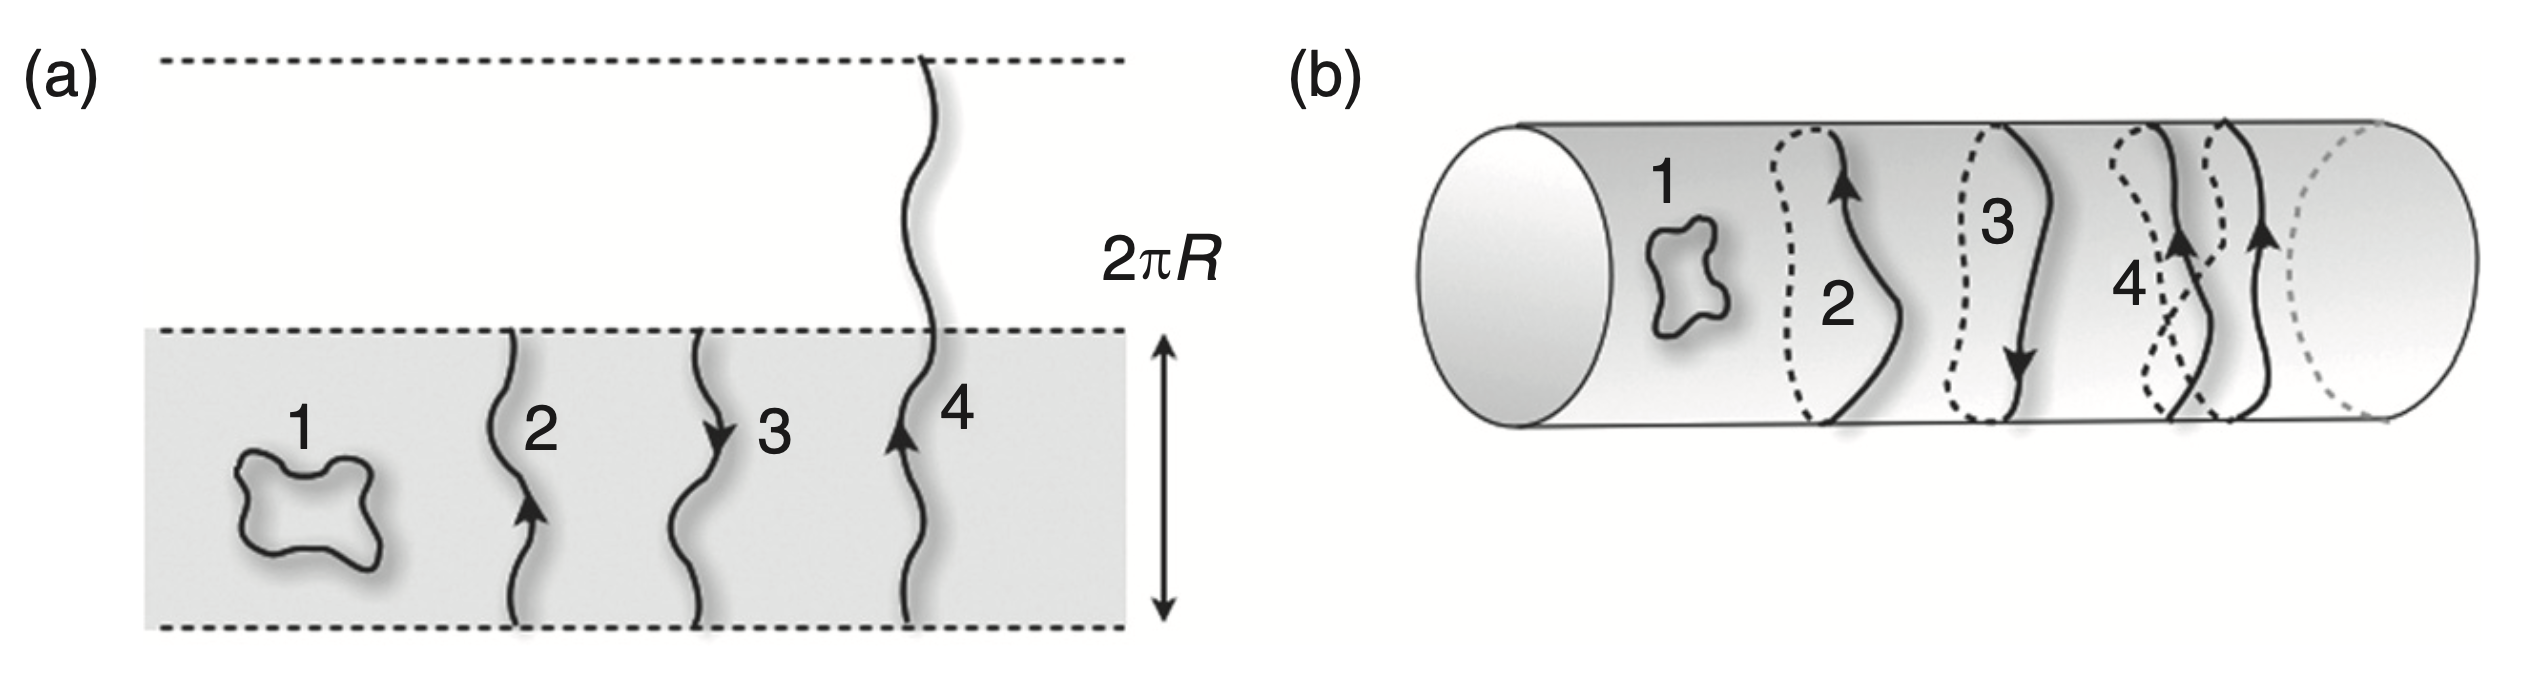
\includegraphics[width=\textwidth]{figures/winding.png}
    \caption{Closed stirng states in $S^1$ compactifications. The closed string $1$ is closed already in flat $26d$ space, and has no winding. Closed strings $2$, $3$ and $4$ are closed only after periodic identification defining the circle. States $2$ and $3$ have opposite winding numbers $\omega = \pm 1$, and state $4$ has a multiple winding $\omega = 2$.}
    \label{fig:winding}
\end{figure}

To express it in terms of the oscillator modes, we first need to specify the boundary conditions. In particular, writing $X^{\hat{i}} = (X^i, X^{25})$, we have the usual periodic boundary condition for the $X^i$ with $i = 2, \dots, 24$, while $X^{25}$ can have a more general boundary condition due to the periodicity $x^{25} = y \simeq y + 2\pi R$ in the internal space. Specifically,
\begin{subequations}
\begin{align}
    X^i(t,\sigma + l) &= X^i(t,\sigma), \quad i = 2, \dots, 24\\
    X^{25}(t,\sigma + l) &= X^{25}(t,\sigma) + 2\pi R \omega, \quad \omega \in \Z.
\end{align}
\end{subequations}
For $\omega = 0$, it describes the usual boundary condition, while for $\omega \neq 0$ it describes a closed string winding around $S^1$ $\omega$-times, as showed in figure~\ref{fig:winding}.

Since the $X^i$ with $i= 2, \dots, 24$ has the same boundary conditions as before, their mode expansion is unchanged, i.e, is given by~\eqref{eq:mode-expansion}, with $\mu = i$ and $\alpha^i_0 = \tilde{\alpha}^i_0 = \sqrt{\frac{\alpha'}{2}}p^i$, i.e,
\begin{subequations}\label{eq:lightcone-mode-decomposition}
\begin{align}
    X^i_L(\xi^+) &= \frac{x^i}{2} + \frac{\alpha'\pi}{l} p^i \xi^+ + i \sqrt{\frac{\alpha'}{2}} \sum_{n\neq 0} \frac{\tilde{\alpha}^i_n}{n}e^{-\frac{2\pi i}{l}n \xi^+}, \\
    X^i_R(\xi^-) &= \frac{x^i}{2} + \frac{\alpha'\pi}{l} p^i \xi^- + i \sqrt{\frac{\alpha'}{2}} \sum_{n\neq 0} \frac{{\alpha}^i_n}{n}e^{-\frac{2\pi i}{l}n \xi^-} .
\end{align}
\end{subequations}

Conversely, the new boundary condition for $X^{25}$ allows for a different expansion. In particular, recalling the generic expansion~\eqref{eq:generic-expansion}, we find
\begin{equation}
    X^{25} (\tau,\sigma) = x^{25} + \sqrt{2\alpha'} \frac{\pi}{l} (\tilde{\alpha}^{25}_0 + \alpha^{25}_0) \tau + \sqrt{2\alpha'} \frac{\pi}{l} (\tilde{\alpha}^{25}_0 - \alpha^{25}_0) \sigma + \textup{oscillators},
\end{equation}
so that, after $\sigma \to \sigma + l$, in order to have $\delta X^{25} = 2\pi R \omega$, we must impose
\begin{equation}\label{eq:equation1}
    \delta X^{25} = \sqrt{2\alpha'} \frac{\pi}{l} (\tilde{\alpha}^{25}_0 - \alpha^{25}_0) l \overset{\mathrm{!}}{=} 2 \pi R \omega \iff \tilde{\alpha}^{25}_0 - \alpha^{25}_0 = \sqrt{\frac{2}{\alpha'}} R \omega, \quad \omega \in \Z.
\end{equation}

Moreover, since we identified $X^{25} \sim X^{25} + 2 \pi R \omega$, in order for the wavefunction $e^{ip_{25}X^{25}}$ to be single-valued the momentum must be quantized, i.e,
\begin{equation}
    p_{25} = \frac{s}{R}, \quad s \in \Z.
\end{equation}
Then, recalling the expression for the Noether's charge associated to spacetime translations, eq.~\eqref{eq:noteher-momentum}, we get
\begin{equation}\label{eq:equation2}
    p^{25} = \frac{1}{\sqrt{2\alpha'}}(\tilde{\alpha}^{25}_0 + \alpha^{25}_0) \overset{\mathrm{!}}{=} \frac{s}{R} \iff \tilde{\alpha}^{25}_0 + \alpha^{25}_0 = \sqrt{2\alpha'} \frac{s}{R}, \quad s \in \Z.
\end{equation}

Solving~\eqref{eq:equation1} and~\eqref{eq:equation2} for $\tilde{\alpha}^{25}_0$ and ${\alpha}^{25}_0$, we get
\begin{equation}
    \tilde{\alpha}^{25}_0 = \sqrt{\frac{\alpha'}{2}} \left( \frac{s}{R} + \frac{\omega R}{\alpha'} \right), \quad {\alpha}^{25}_0 = \sqrt{\frac{\alpha'}{2}} \left( \frac{s}{R} - \frac{\omega R}{\alpha'} \right), \quad \omega, s \in \Z.
\end{equation}

Now, we can perform the same computation which led to~\eqref{eq:level-matching} and~\eqref{eq:mass-shell}, to find that the \emph{level-matching} condition now reads
\begin{equation}\label{eq:comp-level-matrching}
    \tilde{N}_\perp - N_\perp + s \omega = 0, \quad s,\omega \in \Z,
\end{equation}
where the transverse number operators~\eqref{eq:def-transverse-number-op} are defined as before, i.e.,
\begin{equation}\label{eq:equation3}
    \tilde{N}_\perp = \sum_{n> 0} \tilde{\alpha}^{\hat{i}}_{-n}\tilde{\alpha}^{\hat{i}}_n, \quad N_\perp = \sum_{n>  0} \alpha^{\hat{i}}_{-n}\alpha^{\hat{i}}_n.
\end{equation}

Further, \emph{mass-shell} condition in \emph{the $25d$ space $\M_{25}$} reads\footnote{Pay attention to the fact that we're only focusing on $\M_{25}$. Indeed, we compute $-p_\mu p^\mu$, with $\mu = 0, \dots, 24$, \emph{not} $-p_{\hat{\mu}}p^{\hat{\mu}}$, with $\hat{\mu} = 0, \dots, 25$.}
\begin{equation}\label{eq:comp-mass-shell}
    M^2 = - p_\mu p^\mu = \frac{s^2}{R^2} + \frac{\omega^2 R^2}{\alpha'^2} + \frac{2}{\alpha'} (N + \tilde{N} - 2) .
\end{equation}

\begin{mdframed}
\begin{innerproof}
    Once again, the starting point is the relation~\eqref{eq:minus-oscillators} for $n=0$, which, using $\tilde{\alpha}^-_0 = \alpha^-_0 = \sqrt{\frac{\alpha'}{2}}p^-$ and~\eqref{eq:ordering-constants}, reads
    \begin{equation*}
    \begin{aligned}
        p^+p^- &= \frac{1}{\alpha'} \left( \alpha^{\hat{i}}_0 \alpha^{\hat{i}}_0 + \normord{\sum_{n \neq 0}\alpha^{\hat{i}}_{-n}\alpha^{\hat{i}}_n} - 2 \right) = \frac{1}{\alpha'} \left( \alpha^{{i}}_0 \alpha^{{i}}_0 + \alpha^{25}_0 \alpha^{25}_0 + 2 \sum_{n>  0} \alpha^{\hat{i}}_{-n}\alpha^{\hat{i}}_n - 2 \right) \\
        p^+p^- &= \frac{1}{\tilde{\alpha}'} \left( \tilde{\alpha}^{\hat{i}}_0 \tilde{\alpha}^{\hat{i}}_0 + \normord{\sum_{n \neq 0}\tilde{\alpha}^{\hat{i}}_{-n}\tilde{\alpha}^{\hat{i}}_n} - 2 \right) = \frac{1}{\tilde{\alpha}'} \left( \tilde{\alpha}^{{i}}_0 \tilde{\alpha}^{{i}}_0 + \tilde{\alpha}^{25}_0 \tilde{\alpha}^{25}_0 + 2 \sum_{n> 0} \tilde{\alpha}^{\hat{i}}_{-n}\tilde{\alpha}^{\hat{i}}_n - 2 \right) .
    \end{aligned}
    \end{equation*}
    Using, now~\eqref{eq:equation3} and
    \begin{equation*}
        \alpha^i_0 = \tilde{\alpha}^i_0 = \sqrt{\frac{\alpha'}{2}}p^i, \quad \tilde{\alpha}^{25}_0 = \sqrt{\frac{\alpha'}{2}} \left( \frac{s}{R} + \frac{\omega R}{\alpha'} \right), \quad {\alpha}^{25}_0 = \sqrt{\frac{\alpha'}{2}} \left( \frac{s}{R} - \frac{\omega R}{\alpha'} \right), 
    \end{equation*}
    we get
    \begin{equation*}
    \begin{aligned}
        p^+p^- &= \frac{1}{2} p^i p^i + \frac{1}{2} \left( \frac{s}{R} - \frac{\omega R}{\alpha'} \right)^2 + \frac{2}{\alpha'} N - \frac{2}{\alpha'} ,\\
        p^+p^- &= \frac{1}{2} p^i p^i + \frac{1}{2} \left( \frac{s}{R} + \frac{\omega R}{\alpha'} \right)^2 + \frac{2}{\alpha'} \tilde{N} - \frac{2}{\alpha'} .
    \end{aligned}
    \end{equation*}
    Then, by comparison, the new level-matching condition is
    \begin{equation*}
        \frac{1}{2} \left( \frac{s}{R} - \frac{\omega R}{\alpha'} \right)^2 + \frac{2}{\alpha'} N = \frac{1}{2} \left( \frac{s}{R} + \frac{\omega R}{\alpha'} \right)^2 + \frac{2}{\alpha'} \tilde{N} \iff \tilde{N} - N + s \omega  = 0,
    \end{equation*}
    in agreement with~\eqref{eq:comp-level-matrching}. Finally, to find the mass-shell condition, we sum the above relations to obtain
    \begin{equation*}
        2p^+p^- = p^i p^i + \frac{1}{2} \left( \frac{s}{R} + \frac{\omega R}{\alpha'} \right)^2 + \frac{1}{2} \left( \frac{s}{R} - \frac{\omega R}{\alpha'} \right)^2 + \frac{2}{\alpha'} (N + \tilde{N} - 2),
    \end{equation*}
    so that
    \begin{equation}
        M^2 = -p_\mu p^\mu = 2 p^+ p^- - p^i p^i = \frac{s^2}{R^2} + \frac{\omega^2 R^2}{\alpha'^2} + \frac{2}{\alpha'} (N + \tilde{N} - 2),
    \end{equation}
    in agreement with~\eqref{eq:comp-mass-shell}
\end{innerproof}
\end{mdframed}

For future convenience, let's define
\begin{equation}
    \tilde{\alpha}^{25}_0 \equiv \sqrt{\frac{\alpha'}{2}} p_L, \quad {\alpha}^{25}_0 \equiv \sqrt{\frac{\alpha'}{2}} p_R, \quad p_L \equiv \left( \frac{s}{R} + \frac{\omega R}{\alpha'} \right), \quad p_R \equiv \left( \frac{s}{R} - \frac{\omega R}{\alpha'} \right) ,
\end{equation}
so that we can divide the expansion of $X^{25}$ into a left- and a right- moving part, i.e,
\begin{subequations}
\begin{align}
    X^{25}(\tau,\sigma) &= X^{25}_L(\xi^+) + X^{25}_R(\xi^-) \\
    X^{25}_L(\xi^+)     &= \frac{x^{25}}{2} + \frac{\alpha' \pi}{l} p_L \xi^+ + i \sqrt{\frac{\alpha'}{2}} \sum_{n\neq 0} \frac{\tilde{\alpha}^{25}_n}{n}e^{-\frac{2\pi i}{l}n \xi^+} \\
    X^{25}_R(\xi^-)     &= \frac{x^{25}}{2} + \frac{\alpha' \pi}{l} p_R \xi^- + i \sqrt{\frac{\alpha'}{2}} \sum_{n\neq 0} \frac{{\alpha}{25}_n}{n}e^{-\frac{2\pi i}{l}n \xi^-}.
\end{align}
\end{subequations}

Without delving into the details, the Hamiltonian of the system splits into a left and a right part, which are completely independent. So, we can carry out the quantization of the left and right moving coordinates independently, with mass-shell conditions
\begin{equation}
    M^2_L = \frac{p_L}{2} + \frac{2}{\alpha'}(\tilde{N}-1), \quad M^2_R = \frac{p_R}{2} + \frac{2}{\alpha'}({N}-1)
\end{equation}
and only at the end combine the two sectors using the level-matching condition
\begin{equation}
    M^2_L = M^2_R, \quad M^2 = M^2_L + M^2_R .
\end{equation}
This implies that the $2d$ field theory of purely left-moving and purely right-moving fields make sense independently.

Finally, the spectrum is built from the vacuum defined as
\begin{equation}
    ,
\end{equation}
by acting with $.$ in all possible ways.


\section{T-duality}
In the \emph{large volume approx}~\eqref{eq:large-volume-approx}, the non-zero winding states are very massive and decouple. Further, for the remaining zero-winding states, with $\omega = 0$, We recover the Kaluza-Klein description,
\begin{equation}
    m_s^2 = M^2 + \left(\frac{s}{R}\right)^2, \quad M^2 = \frac{2}{\alpha'} (N + \tilde{N} - 2)
\end{equation}

Moreover, one can easily see that the mass-formula~\eqref{eq:comp-mass-shell} is invariant under the so-called \emph{T-duality transformation}
\begin{equation}
    R \to \frac{\alpha'}{R}, \quad s \leftrightarrow \omega .
\end{equation}
Then, the complete spectrum of the theory at radius $R$ is the same as the spectrum of the theory at radius $R' = \frac{\alpha'}{R}$, up to a relabelling of $s$ and $\omega$.

An important consequence of T-duality is that the $R \to 0$ limit corresponds to a decompactification limit of the T-dual theory, in which $R' \to \infty$, so the infinite tower of winding states becoming light in the $R \to 0$ limit are interpreted as an infinite tower of Kaluza-Klein modes becoming light in the $R' \to \infty$ limit.

From the point of view of the coordinates, we can define a T-duality operation as a \emph{parity operation on right movers}. In particular, one can show that T-duality is \emph{not} an accidental property of the spectrum, since the t-dual theories are described by exactly the same wordsheet theory, and differ on how the spacetime geometry is recovered from it. In particular, turning back to the quantized theory in lightcone gauge, we observe that 

\chapter{Type II String}
%**************** RNS SUPERSTRING *********************
\section{Ramond-Neveu-Schwarz Superstring}
We use mostly plus metric $\eta = \textup{diag}(-, +, \dots, +)$ and focus on closed strings. We already focus on the critical string, considering as a background the flat $10$d Minkowski spacetime $\M_{10}$. The worldsheet coordinates are $\xi^a$, $a = 1,2$, where $\sigma \in (0,l)$.

The supersymmetric extension of Polyakov action~\eqref{eq:polyakov-action} is reached by enlarge the field content of the theory. In particular, the idea is to supersymmetrize and couple the $10$ bosonic fields on the worldsheet, $X^\mu (\xi^a)$, $\mu = 0, \dots, 9$, to two-dimensional supergravity. The result are additional worldsheet spinors, which are the superpartners of the $X^\mu$, and will be denoted by $\psi^\mu (\xi^a)$, where the spinorial indices are suppressed. They are taken to be \emph{Majorana-Weyl spinors}.

In particular, in dimension $d=2$ the Clifford algebra reads
\begin{equation}
    \{ \gamma^a, \gamma^b \}_{AB} = 2 \eta^{ab} \1_{AB},
\end{equation}
with $\alpha,\beta = 0, 1$ are the worldsheet indices, while $A,B = 1,2$ the spinorial representation indices. Indeed, in $d=2$, the spinor representation turns out to be two-dimensional as well. A basis for the $\gamma$-matrices is
\begin{equation}
    \gamma^0 = \begin{pmatrix}
        0 & 1 \\
        -1 & 0
    \end{pmatrix}, \quad \gamma^1 = \begin{pmatrix}
        0 & 1 \\
        1 & 0
    \end{pmatrix}
\end{equation}
Further, in $d=2$, the Majorana condition is equivalent to the requirement that the spinors are real i.e.,
\begin{equation}
    \psi = \begin{pmatrix}
        \psi_+ \\ \psi_-
    \end{pmatrix} = \begin{pmatrix}
        \psi^*_+ \\ \psi^*_-
    \end{pmatrix} = \psi^*,
\end{equation}
while the chirality distinguishes between the two inequivalent Weyl representations. In particular, defining the chirality operator $\gamma = \gamma^0 \gamma^1$, we have
\begin{equation}
    \gamma \begin{pmatrix}
        \psi_+ \\ 0
    \end{pmatrix} = \begin{pmatrix}
        \psi_+ \\ 0
    \end{pmatrix}, \quad \gamma \begin{pmatrix}
        0 \\ \psi_-
    \end{pmatrix} = - \begin{pmatrix}
        0 \\ \psi_-
    \end{pmatrix}.
\end{equation}
The two condition are compatible for $d = 2 \mod 8$, dimensions in which Majorana-Weyl spinors exist.

Skipping the details, the classical RNS action adds a Majorana-Weyl spinor for each scalar field. After gauge-fixing the superconformal symmetry to $\gamma_{ab} = \eta_{ab}$, and considering a flat spacetime metric $g_{\mu\nu} = \eta_{\mu\nu}$, it reads
\begin{equation}\label{eq:superstring-action}
    S = -\frac{1}{4\pi} \int_\Sigma \ud^2 \xi \left( \frac{1}{\alpha'} \de_a X^\mu \de^a X_\mu + i \bar{\psi}^\mu_A \gamma^a_{AB} \de_a \psi_\mu \right),
\end{equation}
where the spinor conjugate is defined by
\begin{equation}
    \bar{\psi} \equiv \psi^\dagger \gamma^0 = \psi^T \gamma^0 = (-\psi_-, \psi_+).
\end{equation}

Looking at the mass dimensions, we have
\begin{equation}
     [\psi] = \frac{1}{2}, \quad [X] = -1 .
\end{equation}
It's equations of motion are
\begin{equation}\label{eq:supestring-eom}
    \de_a \de^a X^\mu = 0, \quad \gamma^a \de_a \psi^\mu = 0.
\end{equation}

Taking \emph{worldsheet lightcone coordinates}, $\xi^\pm = \tau \pm \sigma$, the action~\eqref{eq:superstring-action} reads
\begin{equation}
    S = \frac{1}{\pi} \int \ud^2 \xi \left( \frac{1}{\alpha'} \de_+ X \cdot \de_- X + \frac{i}{2} (\psi_+ \cdot \de_- \psi_+ + \psi_- \cdot \de_+ \psi_-) \right) ,
\end{equation}
while the equations of motion~\eqref{eq:supestring-eom} become
\begin{equation}\label{eq:superstring-lightcone-eom}
    \de_+ \de_- X^\mu = 0, \quad \de_- \psi^\mu_+ = \de_+ \psi^\mu_- = 0 .
\end{equation}
This means that in lightcone coordinates we have 
\begin{equation}\label{eq:ligthcone-coordinates-split}
    X^\mu (\xi^\pm) = X^\mu_L (\xi^+) + X^\mu_R(\xi^-), \quad \psi^\mu_+ (\xi^\pm) = \psi^\mu_+ (\xi^+), \quad \psi^\mu_- (\xi^\pm) = \psi^\mu_- (\xi^-) .
\end{equation}

The residual symmetries after gauge fixing the superconformal symmetry have conserved currents
\begin{equation}
\begin{aligned}
    T_{\pm\pm} = -\frac{1}{\alpha'} \de_\pm X \cdot \de_\pm X - \frac{i}{2} (\psi^\mu)_\pm \de_\pm (\psi_\mu)_\pm , \\
    J_\pm = - \sqrt{\frac{1}{2\alpha'}} (\psi^\mu)_\pm \de_\pm X_\mu.
\end{aligned}
\end{equation}
Then, \emph{gauge-fixing} is achieved by imposing the \emph{superconformal Virasoro constraints}
\begin{equation}
    T_{\pm\pm} = , \quad J_{\pm} = 0
\end{equation}
on the equations of motion. 

Let's turn to the mode expansion. Because of~\eqref{eq:ligthcone-coordinates-split}, for the bosonic sector the analysis is the same as before. However, while finding the equations of motion~\eqref{eq:supestring-eom} from~\eqref{eq:superstring-action}, other than the conditino $\delta \psi^\mu (\tau_0) = \delta \psi^\mu (\tau_1) = 0$, which is what we impose in a variational principle, we must be sure that the following boundary term vanishes
\begin{equation}
    \delta S = \frac{1}{2\pi} \int_{\tau_0}^{\tau_1} \ud \tau \left( \psi_+ \cdot \delta \psi_+ - \psi_- \cdot \delta \psi_- \right) \Big|_{\sigma = 0}^{\sigma = l}\overset{\mathrm{!}}{=} 0.
\end{equation}
For the closed string, in which we have periodicity $\sigma \sim \sigma + l$, the above condition is satisfied for
\begin{equation}
\begin{aligned}
    \psi^\mu_+ (\sigma) &= \pm \psi^\mu_+ (\sigma + l) ,\\
    \psi^\mu_- (\sigma) &= \pm \psi^\mu_- (\sigma + l) ,
\end{aligned}
\end{equation}
with the same conditions on $\delta \psi_\pm$. Indeed, anti-periodic boundary conditions for $\psi_\pm$ are possible since observables are built as fermion bilinears. In particular, periodic boundary conditions are referred as \emph{Ramond} (R) boundary conditions, while anti-periodic ones are called \emph{Neveu-Schwartz} (NS). Therefore, fermions on the worldsheet satisfy
\begin{equation}
    \psi (\sigma +l) = e^{2\pi i \phi} \psi(\sigma), \quad \psi = \begin{cases}
        0, \quad \textup{for R-sector} \\ \frac{1}{2}, \quad \textup{for NS-sector}
    \end{cases}
\end{equation}
where more general phases are not allowed since $\psi$ are real.

The conditions for the two spinor components $\psi_+$ and $\psi_-$ can be chosen independently, but Lorentz invariance requires that in a given sector, fermions fields $\psi^\mu$ have the same boundary condition for all $\mu$. This leads to a total of four possibilities: (R,R), (NS,NS), (NS,R) and (R,NS). One can see that, after quantization, modular invariance requires these different boundary conditions to cohexist within the same theory. Roughly speaking, as we have to sum over different topologies to get a consistent string theory, we need to sum over different topological sectors, i.e., boundary conditions, as well. We won't focus on such details and take them for granted.

The mode expansion for the bosonic coordinates is the same as in section~\ref{sec:bosonic-mode-expansion}, while for the fermions we get
\begin{equation}
\begin{aligned}
    \psi^\mu_+ (\xi^+) = \sqrt{\frac{2\pi}{l}} \sum_{r \in \Z + \phi} \tilde{b}^\mu_r e ^{-\frac{2\pi i}{l} r \xi^+} , \\
    \psi^\mu_- (\xi^-) = \sqrt{\frac{2\pi}{l}} \sum_{r \in \Z + \phi} {b}^\mu_r e ^{-\frac{2\pi i}{l} r \xi^-} ,
\end{aligned}
\end{equation}
where
\begin{equation}\label{eq:phi-sectors}
    \phi = \begin{cases}
        0, \quad \textup{for R-sector} \\
        \frac{1}{2}, \quad \textup{for NS-sector} .
    \end{cases}
\end{equation}

Here, $\phi$ can be chosen independently for the left- and right- movers, and the reality of the Majorana-Weyl spinors translates into
\begin{equation}\label{eq:reality-condition}
    (b^\mu_r)^* = b^\mu_{-r}, \quad (\tilde{b}^\mu_r)^* = \tilde{b}^\mu_{-r}.
\end{equation}

%**************** QUANTUM SUPERSTRING *********************
\section{Quantum Superstring}
We quantize the usual way, by finding the canonical conjugate variables, compute their equal-time Poisson brackets and promoting the latter to commutators and anti-commutators on a Hilbert space. Then, we consider the mode expansions and work out the commutators and anti-commutators of the modes operators. The result is
\begin{subequations}
\begin{align}
    \comm{\alpha^\mu_m}{\alpha^\nu_n} = \comm{\tilde{\alpha}^\mu_m}{\tilde{\alpha}^\nu_n} &= m \delta_{m+n} \eta^{\mu\nu} , \\
    \comm{\alpha^\mu_m}{\tilde{\alpha}^\nu_n} &= 0, \\
    \{ b^\mu_m, b^\nu_n \} = \{ \tilde{b}^\mu_m, \tilde{b}^\nu_n \} &= \delta_{m+n} \eta^{\mu\nu} \label{eq:anticomm-bs} \\
    \{ b^\mu_m, \tilde{b}^\nu_n \} &= 0 \\
    \comm{\alpha^\mu_m}{b^\nu_n} &= 0 .
\end{align}
\end{subequations}
Furter, the reality condition of the fermions, $\psi^*_\pm = \psi_\pm$, translates into
\begin{equation}
    (b^\mu_n)^\dagger = b^\mu_{-n} .
\end{equation}

Without delving into the details, let's consider lightcone quantization, where we define the \emph{spacetime lightcone coordinates}
\begin{equation}
    X^\pm = \frac{1}{\sqrt{2}} (X^0 \pm X^1), \quad \psi^\pm = \frac{1}{\sqrt{2}} (\psi^0 \pm \psi^1),
\end{equation}
and the remaining fields are $X^i_L(\xi^+)$, $X^i_R(\xi^-)$, $\psi^i_+(\xi^+)$ and $\psi^i_-(\xi^-)$, with $i = 2, \dots 9$ in spacetime dimension $D = 10$. As in the bosonic case, we can quantize independently the left- and the right-moving sectors and glue them together at then end. Other than the level-matching condition, there will be additional constraints to be imposed here.

The quantization can be carried independently for the left- and right-moving sectors. If there aren't two options, we suppose to be focusing on the right-moving sector, and that the formulas for the left-moving one are the same up to the substitution of the operators with the tilde ones.

One finds the usual normal ordering constants, which are a priori different for (R) and (NS) sectors. After renormalization, and in the critical setting, we find
\begin{equation}
    a_R = \tilde{a}_R = 0, \quad a_{NS} = \tilde{a}_{NS} = \frac{1}{2} .
\end{equation}
In particular, $a$ is considered to be the sum of the zero point energies of the bosons and of the fermions. The fact that $a_R = 0$ suggests that in the (R) sector, supersymmetry is globally preserved by the boundary conditions of bosons and fermions. Conversely, in the (NS) sectors, the local $2d$ supersymmetry is broken by the different boundary conditions.

Similarly to~\eqref{eq:def-transverse-number-op}, the transverse number operators read
\begin{equation}\label{eq:superstring-transverse-number-op}
\begin{aligned}
    N_\perp = \sum_{n > 0} \alpha_{-n}^i \alpha^i_n + \sum_{k \geq 0 + \phi} k b^i_{-k} b^i_k , \\
    \tilde{N}_\perp = \sum_{n > 0} \tilde{\alpha}_{-n}^i \tilde{\alpha}^i_n + \sum_{k \geq 0 + \phi} k \tilde{b}^i_{-k} \tilde{b}^i_k ,
\end{aligned}
\end{equation}
with $\phi$ given by~\eqref{eq:phi-sectors}, different in (R) and (NS) sectors.


For the mass-shell condition, we have a formula similar to~\eqref{eq:left-right-mass-shell}\footnote{Here we aren't considering compactifications yet, so $s = \omega = 0$, and $p_{L/R} = 0$.}, with two independent contributions, $M^2_L$ for the left-moving sector and $M^2_R$ for the right-moving one. Since the normal ordering constants enter the mass-shell\footnote{Via the normal-ordering of $L_0$ in old covariant quantization, or of the hamiltonian in lightcone quantization.}, we should distinguish between the two sectors. In both cases, the \emph{level-matching condition} reads
\begin{equation}\label{eq:superstring-level-matching}
    M^2_L = M^2_R.
\end{equation}

From now on, we'll focus only on the righ-moving part, the equations for the left-moving being the same but with tilde operators. We'll separately study the vacuum and the spectrum of the (NS) and (R) sectors, gluing them together to find the full spectrum of the closed string.

At the end we will focus on the massless spectrum of the theory, so that they form representations of the little group $SO(8)$ of $SO(1,9)$. Let's denote by $\v$ the vector representation, by $\s$ the positive-chirality spinor representation and by $\c$ the negative-chirality co-spinor representation. Recall that, looking at spinors of $SO(1,D-1)$, we can have Majorana-Weyl spinors, with a number of real degrees of freedom equal to $2^{[\frac{D}{2}]-1}$, for $D = 2 \mod 8$. Moreover, looking at spinors of $SO(D)$, we can have real Weyl spinors for $D = 0 \mod 8$. Therefore, we denote the representations of $SO(8)$ by the number of its real degrees of freedom.

A detailed discussion can be found in the appendix of~\cite{polchisnki:superstrings}, from which we take only the summary tables.
\begin{equation}
    \begin{tabular}{|ccccc|}
    \hline
    \multicolumn{5}{|c|}{$SO(1,d-1)$}                                                                                                              \\ \hline
    \multicolumn{1}{|c|}{$d \mod 8$} & \multicolumn{1}{c|}{Majorana} & \multicolumn{1}{c|}{Weyl}    & \multicolumn{1}{c|}{Majorana-Weyl} & min rep \\ \hline
    \multicolumn{1}{|c|}{$2$}        & \multicolumn{1}{c|}{Yes}      & \multicolumn{1}{c|}{Self}    & \multicolumn{1}{c|}{Yes}           & $1$     \\ \hline
    \multicolumn{1}{|c|}{$3$}        & \multicolumn{1}{c|}{Yes}      & \multicolumn{1}{c|}{-}       & \multicolumn{1}{c|}{-}             & $2$     \\ \hline
    \multicolumn{1}{|c|}{$4$}        & \multicolumn{1}{c|}{Yes}      & \multicolumn{1}{c|}{Complex} & \multicolumn{1}{c|}{-}             & $4$     \\ \hline
    \multicolumn{1}{|c|}{$5$}        & \multicolumn{1}{c|}{-}        & \multicolumn{1}{c|}{-}       & \multicolumn{1}{c|}{-}             & $8$     \\ \hline
    \multicolumn{1}{|c|}{$6$}        & \multicolumn{1}{c|}{-}        & \multicolumn{1}{c|}{Self}    & \multicolumn{1}{c|}{-}             & $8$     \\ \hline
    \multicolumn{1}{|c|}{$7$}        & \multicolumn{1}{c|}{-}        & \multicolumn{1}{c|}{-}       & \multicolumn{1}{c|}{-}             & $16$    \\ \hline
    \multicolumn{1}{|c|}{$8$}        & \multicolumn{1}{c|}{Yes}      & \multicolumn{1}{c|}{Complex} & \multicolumn{1}{c|}{-}             & $16$    \\ \hline
    \multicolumn{1}{|c|}{$8+1 = 9$}  & \multicolumn{1}{c|}{Yes}      & \multicolumn{1}{c|}{-}       & \multicolumn{1}{c|}{-}             & $16$    \\ \hline
    \multicolumn{1}{|c|}{$8+2=10$}   & \multicolumn{1}{c|}{Yes}      & \multicolumn{1}{c|}{Self}    & \multicolumn{1}{c|}{Yes}           & $16$    \\ \hline
    \multicolumn{1}{|c|}{$8+3=11$}   & \multicolumn{1}{c|}{Yes}      & \multicolumn{1}{c|}{-}       & \multicolumn{1}{c|}{-}             & $32$    \\ \hline
    \multicolumn{1}{|c|}{$8+4=12$}   & \multicolumn{1}{c|}{Yes}      & \multicolumn{1}{c|}{Complex} & \multicolumn{1}{c|}{-}             & $64$    \\ \hline
    \end{tabular}
\end{equation}
\begin{equation}
    \begin{tabular}{|cccc|}
    \hline
    \multicolumn{4}{|c|}{$SO(d)$}                                                                                 \\ \hline
    \multicolumn{1}{|c|}{$d \mod 8$} & \multicolumn{1}{c|}{Real}   & \multicolumn{1}{c|}{Weyl}    & Real and Weyl \\ \hline
    \multicolumn{1}{|c|}{$0$}        & \multicolumn{1}{c|}{Yes}    & \multicolumn{1}{c|}{Self}    & Yes           \\ \hline
    \multicolumn{1}{|c|}{$1$}        & \multicolumn{1}{c|}{Yes}    & \multicolumn{1}{c|}{-}       & -             \\ \hline
    \multicolumn{1}{|c|}{$2$}        & \multicolumn{1}{c|}{Yes}    & \multicolumn{1}{c|}{Complex} & -             \\ \hline
    \multicolumn{1}{|c|}{$3$}        & \multicolumn{1}{c|}{Pseudo} & \multicolumn{1}{c|}{-}       & -             \\ \hline
    \multicolumn{1}{|c|}{$4$}        & \multicolumn{1}{c|}{Pseudo} & \multicolumn{1}{c|}{Self}    & -             \\ \hline
    \multicolumn{1}{|c|}{$5$}        & \multicolumn{1}{c|}{Pseudo} & \multicolumn{1}{c|}{-}       & -             \\ \hline
    \multicolumn{1}{|c|}{$6$}        & \multicolumn{1}{c|}{Yes}    & \multicolumn{1}{c|}{Complex} & -             \\ \hline
    \multicolumn{1}{|c|}{$7$}        & \multicolumn{1}{c|}{Yes}    & \multicolumn{1}{c|}{-}       & -             \\ \hline
    \end{tabular}
\end{equation}

Let's now analyse the (NS) and (R) sectors.

%**************** ns sector *********************
\subsection{NS Sector.}
We focus on the right-moving sector. Here, $\phi = 1/2$ and $a_{NS} = 1/2$. The \emph{mass-shell condition} reads
\begin{equation}\label{eq:NS-mass-shell}
    \frac{\alpha' M^2_R}{2} = {N}_\perp - \frac{1}{2},
\end{equation}
with number operator given by~\eqref{eq:superstring-transverse-number-op}.

The spectrum is built by defining a groundstate $\ket{0;k}_{NS}$ with spacetime momenta $k_i$, and annihilated by all positive mode operators, i.e.,
\begin{equation}
\begin{aligned}
    b^i_{k +1/2} \ket{0;k}_{NS} &= 0, \quad \forall k \geq 0, \\
    \alpha^i_n \ket{0;k}_{NS} &= 0, \quad \forall n > 0. \\
\end{aligned}
\end{equation}

Then, we apply negative mode operators in all possible ways. Note that there's no zero mode $b^i_0$. Taking for simplicity zero spacetime momentum, the lightest right-moving states are
\begin{equation}\label{eq:table-NS}
\begin{tabular}{|c|c|c|} \hline
    State & $\alpha' M^2_R / 2$ & $SO(8)$ \\ \hline
    $\ket{0}_{NS}$   & $-1/2$   & $\i$   \\ \hline
    $b^i_{-1/2} \ket{0}_{NS}$   & $0$   & $\v$  \\ \hline
\end{tabular}
\end{equation}

%**************** r sector *********************
\subsection{R Sector.}
We focus on the right-moving sector. Here, $\phi = 0$ and $a_R = 0$. The mass-shell condition reads
\begin{equation}\label{eq:R-mass-shell}
    \frac{\alpha' M^2_R}{2} = N_\perp,
\end{equation}
with number operator given by~\eqref{eq:superstring-transverse-number-op}.

The ground state is now $\ket{0}_R$, with $M_R^2 = 0$\footnote{Beware the notation! The $R$ in the mass stands for right-component, \emph{not} Ramond.}. However, we must pay attention to the existence of zero-modes $b^i_0$. Indeed, since $\comm{M^2_R}{b^i_0} = 0$, the application of $b^i_0$ on the ground state does not change its mass. Hence, it is \emph{degenerate}, and we must find how fermionic mode operators act on them. Indeed, we can require that all positive mode operators annihilate it, but we can't consistently require that all the fermionic zero-mode operators annihilate it, since it wouldn't be consistent with the anticommutators
\begin{equation}\label{eq:superstring-clifford}
    \{ b^i_0, b^j_0 \} = \delta^{ij}.
\end{equation}

In particular, the relation~\eqref{eq:superstring-clifford} defines a Cliffod algebra, and defining the action of $b^i_0$ on the degenerate grandstates is equivalent to find a representation for it. To construct such representation, let's recall how to build generic representations for the Clifford algebra.

\begin{mdframed}
The Clifford algebra is defined by
\begin{equation}\label{eq:clifford}
    \{ \Gamma^\mu, \Gamma^\nu \} = 2 \eta^{\mu\nu} , \quad \mu = 0, \dots, 9,
\end{equation}
where we're considering an even dimension $d = 10$, $k=4$. We group the $\Gamma^\mu$ into two sets of $5$ anticommuting raising and lowering operators
\begin{subequations}
\begin{align}
    \Gamma^\pm_0 &= \frac{1}{2} (\pm \Gamma^0 + \Gamma^1), \label{eq:gamma-zero-pm}\\
    \Gamma^\pm_a &= \frac{1}{2}(\Gamma^{2a} \pm i \Gamma^{2a+1}), \quad a = 1, \dots, 4 .\label{eq:gamma-a-pm}
\end{align}
\end{subequations}
They satisfy
\begin{subequations}
\begin{align}
    \{ \Gamma^+_a, \Gamma^-_b \} &= \delta_{ab} , \\
    \{ \Gamma^+_a, \Gamma^+_b \} = \{ \Gamma^-_a, \Gamma^-_b \} &= 0 ,
\end{align}
\end{subequations}
with $a = 0, \dots, 4$. In particular $(\Gamma^+_a)^2=(\Gamma^-_a)^2=0$. So, we can find the lowest weight state by acting repeatedly with the $\Gamma^-_a$ until we reach a spinor annihilated by all of them, i.e.,
\begin{equation}
    \Gamma^-_a \ket{\zeta} = 0, \quad \forall a .
\end{equation}
Then, by starting from $\ket{\zeta}$, we obtain a $2^5 = 32$-dimensional representation by acting with $\Gamma^+_a$, at most once, in all possible ways. We label those states by $\ket{s_0,s_1,s_2,s_3,s_4}$, with $s_a = \pm 1/2$:
\begin{equation}
    \ket{s_0,s_1,s_2,s_3,s_4} \equiv (\Gamma^+_4)^{s_4 + 1/2} (\Gamma^+_3)^{s_3 + 1/2} (\Gamma^+_2)^{s_2 + 1/2} (\Gamma^+_1)^{s_1 + 1/2} (\Gamma^+_0)^{s_0 + 1/2} \ket{\zeta},
\end{equation}
where, in particular,
\begin{equation}
    \ket{\zeta} = \ket{-\frac{1}{2},-\frac{1}{2},-\frac{1}{2},-\frac{1}{2},-\frac{1}{2}}.
\end{equation}

One can verify the Lorentz generators
\begin{equation}
    \Sigma^{\mu\nu} = -\frac{i}{4} \comm{\Gamma^\mu}{\Gamma^\nu}
\end{equation}
indeed satisfy the $SO(1,9)$ algebra, that is,
\begin{equation}
    i \comm{\Sigma^{\mu\nu}}{\Sigma^{\sigma\rho}} = \eta^{\nu\sigma} \Sigma^{\mu\rho} + \eta^{\mu\rho}\Sigma^{\nu\sigma} - \eta^{\nu\rho}\Sigma^{\mu\sigma} - \eta^{\mu\sigma}\Sigma^{\nu\rho}.
\end{equation}
In particular, the generators $\Sigma^{2a,2a+1}$ commute and can be simultaneously diagonalized. In terms of the raising and lowering operators,
\begin{equation}
    S_a \equiv i^{\delta_a} \Sigma^{2a,2a+1} = \Gamma^+_a \Gamma^-_a - \frac{1}{2},
\end{equation}
so that
\begin{equation}
    S_a \ket{s_0,s_1,s_2,s_3,s_4} = s_a \ket{s_0,s_1,s_2,s_3,s_4}.
\end{equation}
The half-integer values show that this is indeed a spinor representation. The spinors form a $2^5 = 32$-dimensional Dirac representation of the Lorentz algebra $SO(1,9)$.

The Dirac representation is reducible as a representation of the Lorentz algebra. Indeed, because $\Sigma^{\mu\nu}$ is quadratic in the $\Gamma$ matrices, the $\ket{s_0,s_1,s_2,s_3,s_4}$ with even or odd numbers of $+\frac{1}{2}$ do not mix. In particular, we can define the chirality matrix 
\begin{equation}
    \Gamma = \Gamma^0 \Gamma^1 \dots \Gamma^9,
\end{equation}
which satisfies
\begin{equation}
    (\Gamma)^2 = 1, \quad \{ \Gamma,\Gamma^\mu \} =0, \quad \comm{\Gamma}{\Sigma^{\mu\nu}} = 0.
\end{equation}
The eigenvalues of $\Gamma$ are $\pm 1$ and one can easily show
\begin{equation}
    \Gamma = 2^5 S_0 S_1 S_2 S_3 S_4 .
\end{equation}
Then, as a matrix acting on $\ket{s_0,s_1,s_2,s_3,s_4}$, $\Gamma$ is diagonal, with matrix element taking the value $+1$ when $s_a$ include an even number of $-1/2$ and $-1$ for an odd number of $-1/2$. It's eigenvalue is called chirality, and the two $2^4 = 16$ states with definite chirality form two inequivalent Weyl representations of the Lorentz algebra. Therefore, for $d=10$, we obtained
\begin{equation}\label{eq:clifford-branch}
    \boldsymbol{32}_\textup{Dirac} = \boldsymbol{16} \oplus \boldsymbol{16'} .
\end{equation}

A priori, the dimensionalities we mentioned above should be regarded as complex. However, in dimensions $d = 2 \mod 8$, we can define Majorana-Weyl spinors. Taking, then, real Majorana spinors from the beginning leads to real degrees of freedom, obviously substituting “Dirac”, with “Majorana”.
\end{mdframed}

Turning back to the string, we notice that~\eqref{eq:superstring-clifford} satisfies~\eqref{eq:superstring-clifford} for $\Gamma^i = \sqrt{2} b^i_0$, and that there are no $0,1$ gamma matrices, since we're in lightcone gauge. Basically, we'll find representations of $SO(8)$, which is the little group for massless representations of $SO(1,9)$.

From a group theoretic point of view the possibility is twofold. On the one hand, we could've started from the old covariant quantization, with anticommutors~\eqref{eq:anticomm-bs} for $m=n=0$,
\begin{equation}
    \{ b^\mu_0, b^\nu_0 \} = \eta^{\mu\nu},
\end{equation}
defining a Clifford algebra for $SO(1,9)$, up to a factor $\sqrt{2}$. Then, similarly to~\eqref{eq:clifford-branch},we'd have found
\begin{equation}
    \boldsymbol{32}_\textup{Majorana} = \boldsymbol{16}_\R \oplus \boldsymbol{16'}_\R ,
\end{equation}
where the degrees of freedom are real and the Majorana spinor decomposes into two set of Weyl spinors with distinct chirality. Further, since we're interested in the little group $SO(8)$, to study the massless spectrum of the superstring, we should've considered the branching
\begin{equation}
\begin{aligned}
    SO(1,9) &\to SO(1,1) \times SO(8) \\
    \boldsymbol{16} &\to (+,\s) \oplus (-,\c) \\
    \boldsymbol{16'} &\to (-,\s) \oplus (+,\c) ,
\end{aligned}
\end{equation}
where $\pm$ denotes two different irreducible representations of $SO(1,1)$. Then we should've applied the physicality condition $G_0\ket{\phi}=0$, to find that the physical state is
\begin{equation}
    \ket{0}_{R} = (+,\s) \oplus (+,\c) .
\end{equation}

On the other hand, and this is what we'll actually do, we can get advantage from the lightcone gauge ad directly find representations of $SO(8)$, focusing on the Clifford algebra~\eqref{eq:superstring-clifford}. As discussed at the beginning of this section, for $SO(8)$ the reality and Weyl conditions are compatible. Indeed, we start from real gamma matrices, due to~\eqref{eq:reality-condition}, and we'll find that the $2^4=16$-dimensional real representation will split into two inequivalent $8$-dimensional real representations of definite chirality.

Let's then focus again on $\Gamma^i = \sqrt{2}b^i_0$. We haven't the matrices $\Gamma^\pm_0$ in eq.\eqref{eq:gamma-zero-pm}, but only~\eqref{eq:gamma-a-pm}, that is
\begin{equation}
    B^\pm_a = \frac{1}{\sqrt{2}} \left( b^{2a}_0 \pm i b^{2a+1}_0 \right), \quad a = 1, \dots, 4.
\end{equation}

Then, the lowest weight state is
\begin{equation}
    B^-_a\ket{0}_{R} = 0, \quad \forall a = 1, \dots, 4,
\end{equation}
which is an eingenstate of the spin operator such that
\begin{equation}
    \ket{0}_{R} = \ket{-\frac{1}{2},-\frac{1}{2},-\frac{1}{2},-\frac{1}{2}},
\end{equation}
with
\begin{equation}
    S_a \ket{s_1,s_2,s_3,s_4} = s_a \ket{s_1,s_2,s_3,s_4}.
\end{equation}

Then, we obtain a $2^4 = 16$-dimensional real representation by application of the $B^+_a$ operators
\begin{equation*}
    \begin{tabular}{|c|c|c|} \hline
        state & eigenstate of $2S_a$ & number of states \\ \hline
        $\ket{0}_{R}$ & $\ket{-,-,-,-}$ & $\binom{4}{0} = 1$ \\ \hline
        \multirow{2}{*}{$B^+_{a_1} \ket{0}_{R}$} & $\ket{+,-,-,-}, \ket{-,+,-,-},$ & \multirow{2}{*}{$\binom{4}{1} = 4$} \\ 
        & $\ket{-,-,+,-}, \ket{-,-,-,+}.$ & \\ \hline
        \multirow{2}{*}{$B^+_{a_1}B^+_{a_2}\ket{0}_{R}$} & $\ket{+,+,-,-}, \ket{+,-,+,-}, \ket{+,-,-,+},$ & \multirow{2}{*}{$\binom{4}{2} = 6$} \\ 
        & $\ket{-,+,+,-}, \ket{-,+,-,+}, \ket{-,-,+,+}.$ & \\ \hline
        \multirow{2}{*}{$B^+_{a_1}B^+_{a_2}B^+_{a_3} \ket{0}_{R}$} & $\ket{-,+,+,+}, \ket{+,-,+,+},$ & \multirow{2}{*}{$\binom{4}{3} = 4$} \\ 
        & $\ket{+,+,-,+}, \ket{+,+,+,-}$ & \\ \hline
        $B^+_{1}B^+_{2}B^+_{3}B^+_{4} \ket{0}_{R}$ & $\ket{+,+,+,+}$ & $\binom{4}{4} = 1$ \\ \hline
    \end{tabular}
\end{equation*}

The states $(\ket{0}_{R}, B^+_{a_1}B^+_{a_2}\ket{0}_{R},B^+_{1}B^+_{2}B^+_{3}B^+_{4} \ket{0}_{R})$ are characterized by an even number of creation operators, so they have positive chirality and gather to form the spinor representation $\s$ of $SO(8)$. Those with negative chirality, namely $(B^+_{a_1} \ket{0}_{R}, B^+_{a_1}B^+_{a_2}B^+_{a_3}\ket{0}_{R})$, form the co-spinor representation $\c$ of $SO(8)$. Recall that the dimensions are real.

In conclusion, the massless modes of (R) sector are\footnote{Again, the R in the mass stands for right-movers, \emph{not} Ramond.}
\begin{equation}\label{eq:table-R}
    \begin{tabular}{|c|c|c|}
        \hline    state & $\alpha' M^2_R / 2$ & $SO(8)$ \\ \hline
        \multirow{2}{*}{$\begin{array}{c} 
            \ket{0}_{R}, B^+_{a_1}B^+_{a_2}\ket{0}_{R}, \\ 
            B^+_{1}B^+_{2}B^+_{3}B^+_{4} \ket{0}_{R} 
        \end{array}$} & \multirow{2}{*}{$0$} & \multirow{2}{*}{$\s$} \\ 
        & & \\ \hline
        $B^+_{a_1} \ket{0}_{R}, B^+_{a_1}B^+_{a_2}B^+_{a_3}\ket{0}_{R}$   & $0$   & $\c$\\ \hline
    \end{tabular}
\end{equation}

For the left-movers the analysis is completely the same, with tilde operators. We need to understand how to glue those sectors together, consistently.

%************** closed string spectrum *****************
\subsection{Closed String Spectrum.}
To obtain the closed string spectrum, we must glue together the left- and the right-moving sectors, constraint by the level-matching condition~\eqref{eq:superstring-level-matching}. Since left and right movers are themselves divided into (R) and (NS) sectors, we have, a priori, $16$ combinations. Basically, we have to look at~\eqref{eq:table-NS} and~\eqref{eq:table-R}, since $\i$ is the only one to have half-integer value for the mass-squared, it can be tensored only with itself to be consistent with~\eqref{eq:superstring-level-matching}. Further, a priori all the massless representations can be tensored, pairwise.

To have a superstring which have spacetime supersymmetry, it's convenient to define $\emph{G-parity}$, and use it in the context of the \emph{GSO-projection}. We're not interested in those details, so we only say that G-parity essentially counts the even-/odd-ness of fermionic excitations. Gathering the information of~\eqref{eq:table-NS} and~\eqref{eq:table-R} into one table, and citing just the result for G-parity, we get the following table, for the right-movers.
\begin{equation*}
\begin{tabular}{|c|c|c|c|c|c|}
  \hline  sector & G-parity & state & little group rep. & $\alpha' M^2_R /2$ & statistics \\ \hline
        NS & $-$ & $\ket{0}_{NS}$   & $SO(9): \i \,$ & $-1/2$ & boson   \\ \hline
    NS & $+$ & $b^i_{-1/2} \ket{0}_{NS}$   & $SO(8): \v$  & 0 & boson \\ \hline 
        \multirow{2}{*}{R} & \multirow{2}{*}{$+$} & \multirow{2}{*}{$\begin{array}{c} 
            \ket{0}_{R}, B^+_{a_1}B^+_{a_2}\ket{0}_{R}, \\ 
            B^+_{1}B^+_{2}B^+_{3}B^+_{4} \ket{0}_{R} 
        \end{array}$} & \multirow{2}{*}{$SO(8): \, \s$} & \multirow{2}{*}{$0$} & \multirow{2}{*}{fermion} \\ 
        & & & & & \\ \hline
        \multirow{2}{*}{R} & \multirow{2}{*}{$-$} & \multirow{2}{*}{$\begin{array}{c} 
            B^+_{a_1} \ket{0}_{R}, \\ 
            B^+_{a_1}B^+_{a_2}B^+_{a_3}\ket{0}_{R}
        \end{array}$} & \multirow{2}{*}{$SO(8): \, \c$} & \multirow{2}{*}{$0$} & \multirow{2}{*}{fermion} \\ 
        & & & & & \\ \hline
       
\end{tabular}
\end{equation*}
For the left-movers the situation is completely analogous.


We'll call NS$_\pm$ and R$_\pm$ the sectors with G-parity $\pm$. Then, the $10$ possibilities to tensor those sectors and glue together left- and right-movers are:
\begin{equation*}
\begin{tabular}{|c|c|c|c|c|c|}
\hline    sector & state rep. & $\alpha' M^2$ & statistics & $SO(8)$ (indices) & $SO(8)$ (dim.)  \\ \hline
    (NS$_-$,NS$_-$) & $\i \otimes \i$ & $-2$ & boson & / & / \\ \hline
    (NS$_+$,NS$_+$) &$\v \otimes \v$&$0$& boson& $[\boldsymbol{0}] \oplus [\boldsymbol{2}] \oplus (\boldsymbol{2})$ &$\boldsymbol{1} \oplus \boldsymbol{28_v} \oplus \boldsymbol{35_v}$\\ \hline
    (R$_+$,R$_+$) &$\s\otimes \s$&$0$& boson & $[\boldsymbol{0}] \oplus [\boldsymbol{2}] \oplus [\boldsymbol{4}]_+$ & $\boldsymbol{1_s} \oplus \boldsymbol{28_s} \oplus \boldsymbol{35_s}$ \\ \hline
    (R$_-$,R$_-$) &$\c \otimes \c$&$0$& boson & $[\boldsymbol{0}] \oplus [\boldsymbol{2}] \oplus [\boldsymbol{4}]_-$ & $\boldsymbol{1_c} \oplus \boldsymbol{28_c} \oplus \boldsymbol{35_c}$\\ \hline
    (R$_-$,R$_+$) &$\c \otimes \s$&$0$& boson & $[\boldsymbol{1}] \oplus [\boldsymbol{3}]$ & $\boldsymbol{8_v} \oplus \boldsymbol{56_v}$\\ \hline
    (R$_+$,R$_-$) &$\s \otimes \c$&$0$& boson& $[\boldsymbol{1}] \oplus [\boldsymbol{3}]$& $\boldsymbol{8_v} \oplus \boldsymbol{56_v}$\\ \hline
    (R$_+$,NS$_+$) &$\s \otimes \v$&$0$& fermion & / & $\c \oplus \boldsymbol{56_s}$\\ \hline
    (R$_-$,NS$_+$) &$\c \otimes \v$&$0$& fermion & / & $\s \oplus \boldsymbol{56_c}$\\ \hline
    (NS$_+$,R$_+$) &$\v\otimes\s$&$0$& fermion & / & $\c \oplus \boldsymbol{56_s}$\\ \hline
    (NS$_+$,R$_-$) &$\v\otimes\c$&$0$& fermion & / & $\s \oplus \boldsymbol{56_c}$ \\ \hline
\end{tabular}
\end{equation*}

In the last two columns, we've decomposed the tensor product representations into irreducible representations of $SO(8)$. In particular, in the second to last column, for the bosons, $(n)$ denotes a symmetric tensor with $n$ indices, while $[n]$ a completely antisymmetric tensor with $n$ indices. Moreover, in the last column, we've counted the \emph{real} degrees of freedom, \emph{on-shell}. Then,
\begin{itemize}
    \item $\i$, $\boldsymbol{28_v}$ and $\boldsymbol{35_v}$ are the usual dilaton $\Phi$, Kalb-Ramond $B_{[ij]}$ and graviton $G_{(ij)}$ in $10$ dimensions;
    \item $\boldsymbol{1_s}$ and $\boldsymbol{1_c}$ represents zero-forms, $C_0$ and $\tilde{C}_0$;
    \item $\boldsymbol{28_s}$ and $\boldsymbol{28_c}$ are the degrees of freedom of two-forms $C_2$ and $\tilde{C}_2$;
    \item $\boldsymbol{35_s}$ and $\boldsymbol{35_c}$ are the degrees of freedom of four-forms $C_4^+$ and $C_4^-$, whose field strenghts are dual and self-dual, respectively;
    \item $\v$ and $\boldsymbol{56}_v$ are the degrees of freedom of a vector and an antisymmetric three tensor, respectively;
    \item $\s$ and $\c$ are the on-shell degrees of freedom of two dilatini of spin $1/2$, one of each handedness;
    \item $\boldsymbol{56}_s$ and $\boldsymbol{56}_c$ are the on-shell degrees of freedom of two gravitini of spin $3/2$, one of each handedness.
\end{itemize}

In particular, for the vector representations $\v \otimes \v$, we used the familiar decomposition
\begin{equation}
    \v \otimes \v = [\boldsymbol{0}] \oplus (\boldsymbol{2}) \otimes [\boldsymbol{2}].
\end{equation}
For the tensor product of two spinor representations, we just cite the group theoretical result, with no proof. For $SO(d)$ in even dimension, with $d = 2l$, the product representations can be decomposed as
\begin{subequations}
\begin{align}
    \boldsymbol{2^{l-1}} \otimes \boldsymbol{2^{l-1}} &= 
    \begin{cases}
        [\boldsymbol{0}] \oplus [\boldsymbol{2}] \oplus \dots \oplus [\boldsymbol{l}]_+, \quad \textup{$l$ even}, \\
        [\boldsymbol{1}] \oplus [\boldsymbol{3}] \oplus \dots \oplus [\boldsymbol{l}]_+, \quad \textup{$l$ odd}, 
    \end{cases} \\
    \boldsymbol{2^{l-1\prime}} \otimes \boldsymbol{2^{l-1\prime}} &= 
    \begin{cases}
        [\boldsymbol{0}] \oplus [\boldsymbol{2}] \oplus \dots \oplus [\boldsymbol{l}]_-, \quad \textup{$l$ even}, \\
        [\boldsymbol{1}] \oplus [\boldsymbol{3}] \oplus \dots \oplus [\boldsymbol{l}]_-, \quad \textup{$l$ odd}, 
    \end{cases}  \\
    \boldsymbol{2^{l-1}} \otimes \boldsymbol{2^{l-1\prime}} &= 
    \begin{cases}
        [\boldsymbol{1}] \oplus [\boldsymbol{3}] \oplus \dots \oplus [\boldsymbol{l-1}], \quad \textup{$l$ even}, \\
        [\boldsymbol{0}] \oplus [\boldsymbol{2}] \oplus \dots \oplus [\boldsymbol{l-1}], \quad \textup{$l$ odd}, 
    \end{cases} 
\end{align}
\end{subequations}
where $[\boldsymbol{n}]_\pm$ denote states which are identified with spacetime fields which are (anti-)self-dual under Hodge star operator.

Applied to our case, in which $d=8$ and $l=4$, we get
\begin{subequations}
\begin{align}
    \s \otimes \s &= [\boldsymbol{0}] \oplus [\boldsymbol{2}] \oplus [\boldsymbol{4}]_+ ,\\
    \c \otimes \c &= [\boldsymbol{0}] \oplus [\boldsymbol{2}] \oplus [\boldsymbol{4}]_-, \\
    \s \otimes \c &= [\boldsymbol{1}] \oplus [\boldsymbol{3}] .\\
\end{align}
\end{subequations}

Finally, for the tensor product of a spinor and vector-bilinears, we get
\begin{subequations}
\begin{align}
    \v \otimes \s = \c \oplus \boldsymbol{56_s} ,\\
    \v \otimes \c = \s \oplus \boldsymbol{56_c} .
\end{align}
\end{subequations}
 
%****************** type ii superstring theories ******************
\subsection{Type II Superstring Theories}
In order to obtain consistent spacetime theories, one should combine the above described sectors in a way which is consistent with CFT on the worldsheet and supersymmetry of spacetime. The mathematical tool to achieve this is the \emph{GSO projection}. Without proving it, we just quote the result, in particular focusing on \emph{type II} theories, which are characterized by $\mathcal{N} = 2$ supersymmetries on spacetime. They're characterized by the sectors
\begin{equation}
\begin{aligned}
   \text{IIA}: \quad &(\text{NS}_+, \text{NS}_+),\; (\text{R}_+, \text{R}_-), \;(\text{NS}_+,\text{R}_-),\; (\text{R}_+, \text{NS}_+) , \\
   \text{IIB}: \quad &(\text{NS}_+, \text{NS}_+), \;(\text{R}_+, \text{R}_+), \;(\text{NS}_+,\text{R}_+), \;(\text{R}_+, \text{NS}_+),
\end{aligned}
\end{equation}
where we could exchange $\text{R}_\pm \to \text{R}_\mp$ in type IIA, and $\text{R}_+\to \text{R}_-$ in type IIB, obtaining equivalent theories in spacetime. The field content from the massless spectrum is the following:
\begin{equation*}
        \begin{tabular}{|ccc|ccc|}
        \hline
        \multicolumn{3}{|c|}{\textbf{Type IIA}} & \multicolumn{3}{c|}{\textbf{Type IIB}} \\ \hline
        \multicolumn{1}{|c|}{sector}  & fields & \multicolumn{1}{|c|}{$SO(8)$} & \multicolumn{1}{l|}{sector}  & fields & \multicolumn{1}{|c|}{$SO(8)$}  \\ \hline
        \multicolumn{1}{|c|}{$(\text{NS}_+, \text{NS}_+)$} & $\Phi$, $B_{[ij]}$, $G_{(ij)}$ & \multicolumn{1}{|c|}{$\v \otimes \v$} & \multicolumn{1}{c|}{$(\text{NS}_+, \text{NS}_+)$}        &      $\Phi$, $B_{[ij]}$, $G_{(ij)}$  & \multicolumn{1}{|c|}{$\v \otimes \v$} \\ \hline
        \multicolumn{1}{|c|}{$(\text{R}_+, \text{R}_-)$} &$C_1$, $C_3$  & \multicolumn{1}{|c|}{$\s\otimes\c$} & \multicolumn{1}{c|}{$(\text{R}_+, \text{R}_+)$}        &    $C_0$, $C_2$, $C_4^+$   & \multicolumn{1}{|c|}{$\s\otimes\s$}  \\ \hline
        \multicolumn{1}{|c|}{$(\text{NS}_+,\text{R}_-)$}        &     $\tilde{\lambda}_a$, $\tilde{\psi}^\mu_a$  & \multicolumn{1}{|c|}{$\v\otimes\c$}  & \multicolumn{1}{c|}{$(\text{NS}_+,\text{R}_+)$}        &     ${\lambda}^{(1)}_a$, ${\psi}^{(1)\mu}_a$  & \multicolumn{1}{|c|}{$\v\otimes\s$}  \\ \hline


        \multicolumn{1}{|c|}{$(\text{R}_+, \text{NS}_+)$}        &     ${\lambda}_a$, ${\psi}^\mu_a$ & \multicolumn{1}{|c|}{$\s\otimes\v$}   & \multicolumn{1}{c|}{$(\text{R}_+, \text{NS}_+)$}        &     ${\lambda}^{(2)}_a$, ${\psi}^{(2)\mu}_a$  & \multicolumn{1}{|c|}{$\s\otimes\v$}  \\ \hline
        \end{tabular}
\end{equation*}

%******************* COMPACTIFICATION OF TYPE II THEORIES
\section{T-duality for Type II Superstrings}
We're now able to generalize the T-duality discussion of section~\ref{sec:t-duality} to Type IIA/IIB superstrings. We focus on the \emph{closed string} and compactify $\M_{10}$ on $\M_{9} \times S^1$. Differently than above, we change the notation for the indices. In particular, we'll denote with $\hat{\mu}$ the indices of $\M_{10}$, with $\hat{\mu} = 0, \dots, 9$, and with $\mu$ the indices of $\M_{9}$, with $\mu = 0, \dots , 8$. This means that we can write $X^{\hat{\mu}} = (X^\mu, X^{9})$. Similarly, the transversal indices will be called $\hat{i}$ in the following, with $\hat{i} = 2, \dots 9$, while $i$ will denote the transversal indices in the non-compact space $\M_{9}$, with $i = 2, \dots 8$. Therefore, in spacetime lightcone coordinates, we have $X^{\hat{\mu}} \to (X^\pm, X^{\hat{i}}) = (X^\pm, X^i, X^{9})$. The same conventions will be used for the fermions on the worldsheet.

An important detail is that the $2$d fermion sector on the worldsheet is completely unchanged by the compactification. Indeed, we suppose that the only effect of the compactification is on the bosonic fields, which describe how the string in embedded in spacetime, while the fermionic fields are added to guarantee worldsheet supersymmetry. Therefore, the fermions will have the usual (R) or (NS) boundary conditions, with no change due to the compactification. For what concerns the bosons, the analysis is parallel to the bosonic string.

Due to the identification $X^9 \simeq X^9 + 2\pi R$, the possible boundary conditions for the bosonic fields are
\begin{equation}
\begin{aligned}
    X^i (\tau, \sigma +l) = X^i(\tau,\sigma), \quad i = 2, \dots, 8, \\
    X^9(\tau,\sigma + l) = X^9(\tau,\sigma) + 2\pi R \omega, \quad \omega \in \Z .
\end{aligned}
\end{equation}
Further, the momentum along $X^9$ is quantized, i.e.,
\begin{equation}
    p_9 = \frac{s}{R}, \quad s \in \Z.
\end{equation}

Regarding the mode decompositions, for $X^i_{L/R}$ it's given by~\eqref{eq:lightcone-mode-decomposition}, with $i = 2, dots, 8$, while for $X^9 (\tau, \sigma) = X^9_L (\xi^+) + X^9_R (\xi^-)$, it reads
\begin{subequations}
\begin{align}
    X^{9}_L(\xi^+)     &= \frac{x^{9}}{2} + \frac{\alpha' \pi}{l} p_{\!_L} \xi^+ + i \sqrt{\frac{\alpha'}{2}} \sum_{n\neq 0} \frac{\tilde{\alpha}^{9}_n}{n}e^{-\frac{2\pi i}{l}n \xi^+} \\
    X^{9}_R(\xi^-)     &= \frac{x^{9}}{2} + \frac{\alpha' \pi}{l} p_{\!_R} \xi^- + i \sqrt{\frac{\alpha'}{2}} \sum_{n\neq 0} \frac{{\alpha}^{9}_n}{n}e^{-\frac{2\pi i}{l}n \xi^-},
\end{align}
\end{subequations}
with
\begin{equation}
    p_{\!_L} \equiv \left( \frac{s}{R} + \frac{\omega R}{\alpha'} \right), \quad p_{\!_R} \equiv \left( \frac{s}{R} - \frac{\omega R}{\alpha'} \right) .
\end{equation}

From~\eqref{eq:left-right-mass-shell},~\eqref{eq:NS-mass-shell} and~\eqref{eq:R-mass-shell}, since the fermions don't enter this analysis, we easily see that the \emph{mass-shell condition} on $\M_9$ reads
\begin{equation}
    M^2_L = \frac{p^2_L}{2} + \frac{2}{\alpha'} \left( \tilde{N}_\perp - \tilde{a}_\phi \right), \quad M^2_R = \frac{p^2_R}{2} + \frac{2}{\alpha'} \left( {N}_\perp - {a}_\phi \right).
\end{equation}
The number operators are given by~\eqref{eq:superstring-transverse-number-op}, i.e.,
\begin{equation}
    \begin{aligned}
        \tilde{N}_\perp = \sum_{n > 0} \tilde{\alpha}_{-n}^i \tilde{\alpha}^i_n + \sum_{k \geq 0 + \phi} k \tilde{b}^i_{-k} \tilde{b}^i_k , \\
        N_\perp = \sum_{n > 0} \alpha_{-n}^i \alpha^i_n + \sum_{k \geq 0 + \phi} k b^i_{-k} b^i_k ,
\end{aligned}
\end{equation}
and $a_\phi$ and $\tilde{a}_\phi$ the ordering constants for the (R) or (NS) sector. In particular, for $\phi = 0$, we have $a_0 = \tilde{a}_0 = a_{R} = 0$, while for $\phi = 1/2$, we get $a_{1/2} = \tilde{a}_{1/2} = a_{NS} = 1/2$.

For a generic $R$, the only massless states are in the sector $(s=0,\omega=0)$. These states correspond to zero modes of the Kaluza-Klein reduction of the effective field theory of $10$d massless modes. Indeed, the internal momentum is zero and there's no winding. Therefore, in order to perform the Kaluza-Klein reduction to $9$d, keeping just the zero-modes, is equivalent to decoupling representations with respect $SO(8)$, the little group for massless representations of $SO(1,9)$ in $\M_{10}$, into representations of $SO(7)$, which is the little group for massless representations of $SO(1,8)$ in $\M_9$.

In particular, looking at (N) and (NS) sectors for left or right movers, separately, we get
\begin{equation}
        \begin{tabular}{|c|c|c|}
     \hline   sector & $SO(8)$ rep. & $SO(7)$ rep.    \\ \hline
        NS$_+$ & $\v$ & $\boldsymbol{7} \oplus \boldsymbol{1}$ \\ \hline
        R$_+$  & $\s$ &$ \boldsymbol{8}  $  \\ \hline
        R$_-$  & $\c$ & $\boldsymbol{8} $ \\\hline                                                
        \end{tabular}
\end{equation}
where $\boldsymbol{1}$ is the scalar representation of $SO(7)$, $\boldsymbol{7}$ is the vector one and $\boldsymbol{8}$ the spinor representation. Notice that, looking at $SO(d)$, for $d = 7 \mod 8$ we can impose the reality condition, but \emph{not} the Weyl one, since there's no chirality in odd dimensions. Therefore, there's a real, non-chiral, spinor representation of $SO(7)$ of dimension $8$ and both $\s$ and $\c$ are decomposed into this $\boldsymbol{8}$.

Then, we have to glue together the left and right movers. To do so, we can decompose the left and right movers with respect to $SO(7)$, separately, and then tensor them\footnote{An equivalent procedure would be to tensor the representations of $SO(8)$ and then decompose them with respect to $SO(7)$. Both methods give the same result.}.
\begin{equation*}
\scalebox{0.89}{
\begin{tabular}{|cccccc|}
    \hline
    \multicolumn{6}{|c|}{Type IIA}                                                                                                                                                                                                                                                                                                                                                                                   \\ \hline
    \multicolumn{1}{|c|}{sector}                           & \multicolumn{1}{c|}{$SO(8)$}                          & \multicolumn{1}{c|}{$10$d fields}                                                        & \multicolumn{1}{c|}{$SO(7)$}                                          & \multicolumn{1}{c|}{$SO(7)$ irrep}                                                    & $9$d fields                          \\ \hline
    \multicolumn{1}{|c|}{\multirow{3}{*}{(NS$_+$,NS$_+$)}} & \multicolumn{1}{c|}{\multirow{3}{*}{$\v \otimes \v$}} & \multicolumn{1}{c|}{\multirow{3}{*}{$\Phi, B_{[\hat{i}\hat{j}]}, G_{(\hat{i}\hat{j})}$}} & \multicolumn{1}{c|}{$\seven \otimes \seven$}                          & \multicolumn{1}{c|}{$\boldsymbol{1} \oplus \boldsymbol{21}\oplus\boldsymbol{27}$}     & $\phi, B_{[ij]}, G_{(ij)}$           \\ \cline{4-6} 
    \multicolumn{1}{|c|}{}                                 & \multicolumn{1}{c|}{}                                 & \multicolumn{1}{c|}{}                                                                    & \multicolumn{1}{c|}{$(\seven \otimes \i) \oplus (\i \otimes \seven)$} & \multicolumn{1}{c|}{$\boldsymbol{7}\oplus \boldsymbol{7}$}                            & $G_{i9}, B_{i9}$                     \\ \cline{4-6} 
    \multicolumn{1}{|c|}{}                                 & \multicolumn{1}{c|}{}                                 & \multicolumn{1}{c|}{}                                                                    & \multicolumn{1}{c|}{$\i \otimes \i$}                                  & \multicolumn{1}{c|}{$\boldsymbol{1}$}                                                 & $G_{99}$                             \\ \hline
    \multicolumn{1}{|c|}{(R$_+$,R$_-$)}                    & \multicolumn{1}{c|}{$\s \otimes \c$}                  & \multicolumn{1}{c|}{$C_{\hat{i}}, C_{[\hat{i}\hat{j}\hat{k}]}$}                          & \multicolumn{1}{c|}{$\eight \otimes \eight$}                          & \multicolumn{1}{c|}{$\i \oplus \seven \oplus \boldsymbol{21} \oplus \boldsymbol{35}$} & $A_9, A_i, C_{9i}, C_{ijk}$          \\ \hline
    \multicolumn{1}{|c|}{\multirow{2}{*}{(NS$_+$,R$_-$)}}  & \multicolumn{1}{c|}{\multirow{2}{*}{$\v \otimes \c$}} & \multicolumn{1}{c|}{\multirow{2}{*}{$\tilde{\lambda}_a, \tilde{\psi}^{\hat{i}}_a$}}      & \multicolumn{1}{c|}{$\seven \otimes \eight$}                          & \multicolumn{1}{c|}{$\boldsymbol{8} \oplus\boldsymbol{48}$}                           & $\tilde{\psi}^i_a, \tilde{\psi}^9_a$ \\ \cline{4-6} 
    \multicolumn{1}{|c|}{}                                 & \multicolumn{1}{c|}{}                                 & \multicolumn{1}{c|}{}                                                                    & \multicolumn{1}{c|}{$\i \otimes \eight$}                              & \multicolumn{1}{c|}{$\eight$}                                                         & $\tilde{\lambda}_a$                  \\ \hline
    \multicolumn{1}{|c|}{\multirow{2}{*}{(R$_+$,NS$_+$)}}  & \multicolumn{1}{c|}{\multirow{2}{*}{$\s\otimes\v$}}   & \multicolumn{1}{c|}{\multirow{2}{*}{${\lambda}_a, {\psi}^{\hat{i}}_a$}}                  & \multicolumn{1}{c|}{$\eight\otimes\seven$}                            & \multicolumn{1}{c|}{$\boldsymbol{8} \oplus\boldsymbol{48}$}                           & $\psi^i_a, \psi^9_a$                 \\ \cline{4-6} 
    \multicolumn{1}{|c|}{}                                 & \multicolumn{1}{c|}{}                                 & \multicolumn{1}{c|}{}                                                                    & \multicolumn{1}{c|}{$\eight \otimes \i$}                              & \multicolumn{1}{c|}{$\eight$}                                                         & $\lambda_a$                          \\ \hline
    \multicolumn{6}{|c|}{Type IIB}                                                                                                                                                                                                                                                                                                                                                                                   \\ \hline
    \multicolumn{1}{|c|}{sector}                           & \multicolumn{1}{c|}{$SO(8)$}                          & \multicolumn{1}{c|}{$10$d fields}                                                        & \multicolumn{1}{c|}{$SO(7)$}                                          & \multicolumn{1}{c|}{$SO(7)$ irrep}                                                    & $9$d fields                          \\ \hline
    \multicolumn{1}{|c|}{\multirow{3}{*}{(NS$_+$,NS$_+$)}} & \multicolumn{1}{c|}{\multirow{3}{*}{$\v \otimes \v$}} & \multicolumn{1}{c|}{\multirow{3}{*}{$\Phi, B_{[\hat{i}\hat{j}]}, G_{(\hat{i}\hat{j})}$}} & \multicolumn{1}{c|}{$\seven \otimes \seven$}                          & \multicolumn{1}{c|}{$\boldsymbol{1} \oplus \boldsymbol{21}\oplus\boldsymbol{27}$}     & $\phi, B_{[ij]}, G_{(ij)}$           \\ \cline{4-6} 
    \multicolumn{1}{|c|}{}                                 & \multicolumn{1}{c|}{}                                 & \multicolumn{1}{c|}{}                                                                    & \multicolumn{1}{c|}{$(\seven \otimes \i) \oplus (\i \otimes \seven)$} & \multicolumn{1}{c|}{$\boldsymbol{7}\oplus \boldsymbol{7}$}                            & $G_{i9}, B_{i9}$                     \\ \cline{4-6} 
    \multicolumn{1}{|c|}{}                                 & \multicolumn{1}{c|}{}                                 & \multicolumn{1}{c|}{}                                                                    & \multicolumn{1}{c|}{$\i \otimes \i$}                                  & \multicolumn{1}{c|}{$\boldsymbol{1}$}                                                 & $G_{99}$                             \\ \hline
    \multicolumn{1}{|c|}{(R$_+$,R$_+$)}                    & \multicolumn{1}{c|}{$\s \otimes \s$}                  & \multicolumn{1}{c|}{$C_0, C_{[\hat{i}\hat{j}]}, C_{[\hat{i}\hat{j}\hat{k}\hat{l}]}^+$}   & \multicolumn{1}{c|}{$\eight \otimes \eight$}                          & \multicolumn{1}{c|}{$\i \oplus \seven \oplus \boldsymbol{21} \oplus \boldsymbol{35}$} & $a, C_{i9}, C_{ij}, C_{ijk9}$        \\ \hline
    \multicolumn{1}{|c|}{\multirow{2}{*}{(NS$_+$,R$_+$)}}  & \multicolumn{1}{c|}{\multirow{2}{*}{$\v \otimes \s$}} & \multicolumn{1}{c|}{\multirow{2}{*}{${\lambda}_a^{(1)}, {\psi}^{(1)\hat{i}}_a$}}         & \multicolumn{1}{c|}{$\seven \otimes \eight$}                          & \multicolumn{1}{c|}{$\boldsymbol{8} \oplus\boldsymbol{48}$}                           & $\psi^{(1)9}_a, \psi^{(1)i}_a$       \\ \cline{4-6} 
    \multicolumn{1}{|c|}{}                                 & \multicolumn{1}{c|}{}                                 & \multicolumn{1}{c|}{}                                                                    & \multicolumn{1}{c|}{$\i \otimes \eight$}                              & \multicolumn{1}{c|}{$\eight$}                                                         & $\lambda^{(1)}_a$                    \\ \hline
    \multicolumn{1}{|c|}{\multirow{2}{*}{(R$_+$,NS$_+$)}}  & \multicolumn{1}{c|}{\multirow{2}{*}{$\s\otimes\v$}}   & \multicolumn{1}{c|}{\multirow{2}{*}{${\lambda}_a^{(2)}, {\psi}^{(2)\hat{i}}_a$}}         & \multicolumn{1}{c|}{$\eight\otimes\seven$}                            & \multicolumn{1}{c|}{$\boldsymbol{8} \oplus\boldsymbol{48}$}                           & $\psi^{(2)9}_a, \psi^{(2)i}_a$       \\ \cline{4-6} 
    \multicolumn{1}{|c|}{}                                 & \multicolumn{1}{c|}{}                                 & \multicolumn{1}{c|}{}                                                                    & \multicolumn{1}{c|}{$\eight \otimes \i$}                              & \multicolumn{1}{c|}{$\eight$}                                                         & $\lambda^{(2)}_a$                    \\ \hline
    \end{tabular}
}
\end{equation*}

Notice that, in decomposing in irreducible representations of $SO(7)$, each representation is labelled by its real dimension, which is equal to the \emph{on-shell} degrees of freedom of the corresponding field. 

For the bosons it's enough to count the number of independent indices, taking into account the symmetry/antisymmetry property. For fermions, one can show that the handedness of the dilatini is opposite to that of the gravitini. Together, a gravitino and a dilatino form a reducible vector-spinor $\psi^\mu_a$ of $SO(1,9)$, where $\mu$ are the spacetime indices while $a$ the spinorial ones. Its traceless part, $\Gamma^\mu \psi_\mu = 0$ it the gravitino, while the trace is the dilatino. Lightcone quantization can be carefully carried over, obtaining, for the gravitino, a state like $\psi^i_a$, but with a constraint deriving from $\Gamma^\mu \psi_\mu = 0$. Without the derivation, we just remark that this constraint will impose $8$ conditions for $SO(8)$ and $SO(7)$, leading to the correct number of degrees of freedom on-shell.

As usual, similarly to~\eqref{eq:radion-and-radius}, the scalar which arise from the metric, i.e., $G_{99}$, sets the volume of extra dimension, namely, the compactification radius in this case. There's, however, another scalar, arising from the R-R sector, which is $A_9$. Then, it would be interesting to describe the compactification for an arbitrary backgorund of this field. Unfortunately, it's not known how to couple R-R fields to the $2$d worldsheet theory.

Recall that NS-NS fields are the same as the bosonic string. For them, we know how to couple the background to the $2$d theory. This is provided by the \emph{non-linear $\sigma$-model} action, which reads
\begin{equation}
    S_\sigma = \frac{1}{4\pi\alpha'} \int_\Sigma \ud^2 \xi \sqrt{-\det \gamma} \left[ \left( \gamma^{ab} G_{\mu\nu}(X) + i \epsilon^{ab} B_{\mu\nu}(X)  \right) \de_a X^\mu \de_b X^\nu + \alpha' \mathcal{R} \phi(X) \right],
\end{equation}
and it's usually exactly solvable. There's no analogue for R-R fields, to couple them directly to the $2$d worldsheet theory. Indeed, they must be coupled to the worldvolume of D-branes, through \emph{Cern-Simons} actions, rising many complications.

The interesting thing to notice is that the $9$d massless spectrum for type IIA and IIB is the same. In particular, chirality of type IIB is lost after compactification, since there's no notion of chirality in odd dimensions. It's easy to see from the $9$d spectrum that the theory has $\mathcal{N} = 2$ susy, since there are two gravitini. The spectrum, indeed, corresponds to $9$d supergravity with $32$ supercharges, which is a unique theory.

In general, \emph{toroidal compactifications} don't break any supersymmetry, and the \emph{number of supercharges is conserved}. Indeed, compactifying on $T^n$ presenrves the spinor degrees of freedom, since the representation of $SO(1,9)$ simply reorganizes under $SO(1,4)$, without loosing degrees of freedom. Then, compactifying type IIA and IIB on $T^6$ to obtain a $4$d spacetime theory, would lead to $\mathcal{N}=8$ $4$d supergravity, since the $32$ supercharges organize into $8$ independent Majorana spinors in $4$d. This is \emph{not} a chiral theory, and so it's useless for phenomenology.

\appendix
\chapter{Group Theory Basics}
This appendix follows Uranga's. It has the purpose of introducing some useful concepts of group theory and their application. It is by no means complete and formal.

%******************** LIE GROUPS AND LIE ALGEBRA *********************
\section{Lie Groups and Lie Algebra}
\paragraph{Lie Groups}
A \emph{Lie Group} $G$ is a group where the elements are labeled by a set of continuous real parameters $\xi^a$, $a = 1 \dots N$, such that
\begin{equation}
    g(\xi) \cdot g(\xi') = g(f(\xi,\xi')),
\end{equation}
where $f^a(\xi,\xi')$ is a continuous function of $\xi,\xi'$. A Lie group is also a differentiable manifold, with $g(\xi=0)=e$, and dimension $\dim{G} = N$.

\paragraph{Group Representations}
A representation is a map $R$ from the group $G$, onto the endomorphisms on a vector space $V$, $\End(V)$, such that each element $g \in G$ is represented by an operator $R(g)$ acting on V and it preserves the group properties, that it
\begin{equation}
\begin{aligned}
    R: G &\to \End(V),  \quad \textup{s.t.} \, R(g \cdot h) = R(g)R(h)\\
       g &\mapsto R(g)
\end{aligned}
\end{equation}
Let $\ket{e_i}$ be a basis of $V$. Then, the matrix elements of $R(g)$ are
\begin{equation}
    R(g)_{ij} = \bra{e_i} R(g) \ket{e_j}.
\end{equation}
A representation is called \emph{reducible} if can be decomposed into block-diagonal form
\begin{equation}
     R(g) = \begin{pmatrix}
        R_1(g) & 0 \\
        0 & R_2(g)
    \end{pmatrix}, \quad \forall g \in G .
\end{equation}

Let's consider two representation spaces $V_1$ and $V_2$, with dimensions $n_1$ and $n_2$ and basis $\ket{e_i}$ and $\ket{f_n}$, respectively. Further, let's consider the representations $R_1: G \to \End(V_1)$ and $R_2: G \to \End(V_2)$. We can define the \emph{direct sum of representations} $R = R_1 \oplus R_2$, of dimension $\dim(R) = n_1 + n_2$, by
\begin{equation}
\begin{aligned}
    R = R_1 \oplus R_2 : G &\to \End(V_1 \oplus V_2) \\
    g &\mapsto R(g) = \begin{pmatrix}
        R_1(g) & 0 \\
        0 & R_2(g)
    \end{pmatrix}
\end{aligned}
\end{equation}
and the \emph{tensor product of representations} $R = R_1 \otimes R_2$, of dimension $\dim(R) = n_1 n_2$, by
\begin{equation}
\begin{aligned}
    R = R_1 \otimes R_2: G &\to \End(V_1 \times V_2) \\
    g &\mapsto R(g)_{in,jm} = R_1(g)_{ij} R_2(g)_{nm}
\end{aligned}
\end{equation}

\paragraph{Lie Algebra}
For a generic Manifold $\M$, the \emph{tangent space} at a point $p \in \M$, $T_p \M$, is defined as the space spanned by $\left. \de_a \right|_p$, $a = 1, \dots, \dim \M$, which are defined by
\begin{equation}
\begin{aligned}
    \left. \de_a \right|_p : \mathcal{F} (\M) &\to \R \\
    f(x) &\mapsto \left. \de_a f(x) \right|_p ,
\end{aligned}
\end{equation}
where $\mathcal{F}$ is the space of functions on $\M$.

Similarly, given a Lie group $G$, we define the \emph{tangent space at the origin} $e = g(\xi=0)$, as the space spanned by $T_a$, $a = 1, \dots, \dim(G)$, defined by
\begin{equation}
\begin{aligned}
    T_a : \mathcal{R}(G) &\to \textup{Mat} \\
    R(g(\xi)) &\mapsto \left. -i \de_a R(g(\xi)) \right|_{\xi=0} .
\end{aligned}
\end{equation}
Here, $\mathcal{R}(G)$ is the space of representations on $G$ and $\textup{Mat}$ it the space of matrices. Formally we could have written
\begin{equation}\label{eq:app-form}
    T_a = \left. -i \de_a g \right|_e
\end{equation}

Given a representation of the group $R: G \to \End(V)$, we define the \emph{representation of the algebra generators in the group's representation $R$} by
\begin{equation}
    t^R_a = \left. -i \de_a R(\xi) \right|_{\xi=0} .
\end{equation}
Finally, the \emph{Lie algebra} $\g$ is the algebra generated by $T_a$, and the generators are $\sum_a \lambda_a T^a$.

\paragraph{Exponential Map}
Formally we can write
\begin{equation}
    g(0,\dots, \delta \xi^a, \dots, 0) = e + (\de_a g)_e \delta \xi^a = e + i T_a \delta X^a,
\end{equation}
where we used~\eqref{eq:app-form}. In any representation $R$ of the group, we could either write
\begin{equation}
\begin{aligned}
    R(0, \dots, \xi^a + \delta \xi^a, \dots 0) &= R(0, \dots, \delta \xi^a, \dots, 0) R(0, \dots, \xi^a, \dots, 0)  \\
    &= \left( 1 + \left. \de_a R\right|_{\xi=0} \delta \xi^a \right) R(0, \dots, \xi^a, \dots, 0) \\
    &= \left( 1 + i t^R_a \delta \xi^a \right) R(0, \dots, \xi^a, \dots, 0)  ,
\end{aligned}
\end{equation}
or
\begin{equation}
    R(0, \dots, \xi^a + \delta \xi^a, \dots, 0) = R(0, \dots, \xi^a, \dots, 0) + \de_a R(0, \dots, \xi^a, \dots, 0) \delta \xi^a ,
\end{equation}
which leads to
\begin{equation}
    \de_a R(0, \dots, \xi^a, \dots, 0) = i t^R_a R(0, \dots, \xi^a, \dots, 0).
\end{equation}
Solving the differential equation, we get
\begin{equation}
    R(0, \dots, \xi^a, \dots, 0) = e^{i t^R_a \xi^a}, \quad \textup{(no sum)},
\end{equation}
or rather, from the formal group,
\begin{equation}
    g(0, \dots, \xi^a, \dots, 0) = e^{i T_a \xi^a} \quad \textup{(no sum)}.
\end{equation}

Then, any group element continuously connected to the identity can be written as
\begin{equation}
    g(\xi) = e^{i T_a \xi^a} .
\end{equation}

\paragraph{Commutation Relations}
The generators satisfy the comutation relations
\begin{equation}
    \comm{T_a}{T_b} = i f_{abc} T_c .
\end{equation}
One can show that the structure constants $f_{abc}$ are determined by the group multiplication law and, conversely, that the group multiplication law determines the structure constants. They satisfy the Jacoby identity
\begin{equation}
    \comm{T_a}{\comm{T_b}{T_c}} + \comm{T_c}{\comm{T_a}{T_b}} + \comm{T_b}{\comm{T_c}{T_a}} = 0
\end{equation}

\paragraph{Algebra Representation}
Given a Lie algebra $\g$, an \emph{algebra representation} $\rho$ is a map from the algebra $\g$ onto the endomorphisms on a vector space $V$, which preserves the comutation relations. In particular, it acts on the generators as
\begin{equation}
\begin{aligned}
    \rho: \g &\to \End(V), \quad \textup{s.t.} \, \comm{t^R_a}{t^R_b} = i f_{abc} t^R_c \\
    T_a &\mapsto \rho(t_a) \equiv t^R_a .
\end{aligned}
\end{equation}

One can prove that given a representation $R$ of the group, one can find the representation of the algebra's generators as 
\begin{equation}
    t^R_a = -i \de_a R(\xi).
\end{equation}
Conversely, given the representation of the generators of the algebra, the group's representation can be found to be
\begin{equation}\label{appeq:rep-ga}
    R(\xi) = e^{i t^R_a \xi^a} .
\end{equation}

By suitably normalizing $\tr(t^R_a t^R_b)$, for any representation $R$ we can find a basis of $\g$ where the structure constants $f_{abc}$ are completely antisymmetric. From now on we consider this case.

Further, from now on we focus on \emph{compact groups}. For them any representation is equivalent to a \emph{unitary representation}, which is a representation with \emph{hermitian generators} and \emph{real structure constants}.

%******************** ADJOINT REPRESENTATION *********************
\section{Adjoint Representation.}
Take a group $G$, with $\dim G = N$ and algebra $\g$ with abstract generators $T_a$, $a = 1, \dots, N$. The \emph{adjoint representation} is a map from the algebra $\g$ onto the endomorphisms of the algebra, $\End(\g)$, such that, for $X = T_a \xi^a \in \g$,
\begin{equation}
\begin{aligned}
    Ad: \g &\to \End(g) \\
    X &\mapsto Ad(X), \quad \textup{s.t.} \, \forall Y \in \g, \, Ad(X)Y = \comm{X}{Y} \\
    T_a &\mapsto Ad(T_a) \equiv t^{Ad}_a, \quad \textup{s.t.} \, \forall T_b \in \g, \, t^{Ad}_a T_b = \comm{T_a}{T_b} = i f_{abc} T_c .
\end{aligned}
\end{equation}
In other words, the representative of $T_a$ is an operator from the algebra onto itself, $t^{Ad}_a: \g \to \g$, with matrix elements
\begin{equation}
    (t^{Ad}_a)_{bc} = -i f_{abc} .
\end{equation}

The dimension of the adjoint representation is the same as the dimension of the group. To have a clearer notation, call the basis of the representation space $\{ \ket{T_a} \}$, $a = 1, \dots, N$. Then, a generator $T_a$ is represented by $t^{Ad}_a$, which is such that
\begin{equation}\label{appeq:adjoint-def}
    t^{Ad}_a \ket{T_b} = \ket{\comm{T_a}{T_b}} = i f_{abc} \ket{T_c}.
\end{equation}


%******************** SU(2) ROOTS AND WEIGHTS *********************
\section{\texorpdfstring{$SU(2)$}{SU(2)} and its Roots and Weights.}
Before turning to the general case, let's consider the group $SU(2)$ and define the roots and the weights. After that, we'll generalize to generic groups. The $SU(2)$ algebra is defined by the commutation relations $\comm{J_a}{J_b} = i \epsilon_{abc} J_c$. 

\paragraph{Roots}
The objective is to put the algebra in the \emph{Cartan-Weyl form}. To do so, we first look for the \emph{Cartan subalgebra}, which is spanned by a \emph{maximal set of mutually commuting generators}. Since for $SU(2)$ all pairs of generators are non-commuting, the maximal set of commuting generators is made of one element, say $J_3$. Then, we rearrange the remaining generators as
\begin{equation}
    J^\pm = \frac{1}{\sqrt{2}} (J_1 \pm i J_2) ,
\end{equation}
such that the commutators become
\begin{subequations}
\begin{align}
    \comm{J_3}{J^\pm} &= \pm J^\pm, \\
    \comm{J_3}{J_3} &= 0 ,\\
    \comm{J^+}{J^-} &= J_3 .
\end{align}
\end{subequations}

\begin{figure}
    \centering
    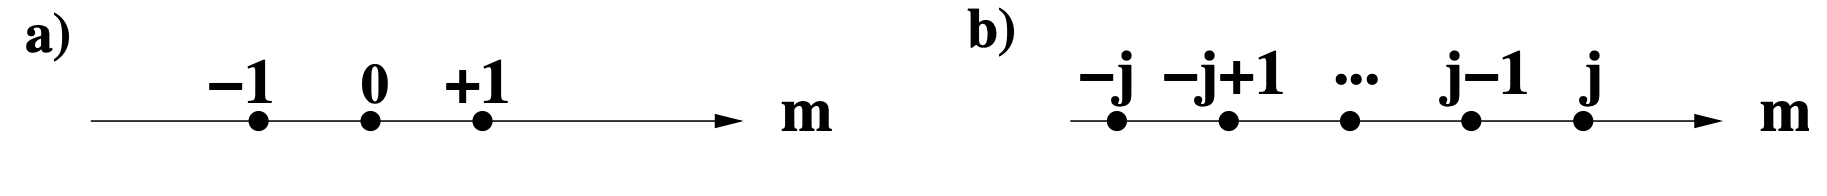
\includegraphics[width=0.75\textwidth]{figures/roots.png}
    \caption{Figure (a) shows the root diagram for the $SU(2)$ Lie algebra. Figure (b) shows the general structure of the weights for irreducible representations of this algebra.}
    \label{fig:su2-root-diagram}
\end{figure}

These relations define the \emph{roots} of the algebra, which is a property independent of the particular representation. However, to understand it better, let's consider the adjoint representation, in which
\begin{subequations}
\begin{align}
    J^{Ad}_3 \ket{J^\pm} &= \pm \ket{J^\pm} \label{appeq:ad1}\\
    J_3^{Ad} \ket{J_3} &= 0 \label{appeq:ad2}\\
\end{align}
\end{subequations}
Focusing on~\eqref{appeq:ad1} and exponentiating it, using~\eqref{appeq:rep-ga} for the left-hand side, we find
\begin{equation}
    g(\xi) \ket{J^\pm} = e^{\pm i \xi J_3} \ket{J^\pm} ,
\end{equation}
which tells us that $\ket{J^\pm}$ transform under the $U(1)$ subgroup generated by the Cartan generator $J_3$, with charges $\pm 1$. Similarly, from~\eqref{appeq:ad2}, $J_3$ has charge $0$. Those charges are called \emph{roots} of the algebra, and in $SU(2)$ case, the charges are $(J_-, J_3, J_+) = (-1,0,1)$. They can be graphically represented in a \emph{root diagram}, as showed in figure~\ref{fig:su2-root-diagram}.

\paragraph{Weights}
Let's now focus on the construction of irreducible representations. The representation space is a vector space spanned by a set of basis vectors. It's then natural to take a basis in which the representative of $J_3$ is diagonal. Then, in this basis, it's natural to label each basis vector by its $J_3$ eigenvalue, that is\footnote{We should write something like $\rho(J_3)$, i.e., we're considering the generator in a particular representation. However, it should be clear from the context whether we're dealing with the abstract generator or its representative in the representation $\rho$.}
\begin{equation}
    J_3 \ket{\mu} = \mu \ket{\mu} .
\end{equation}
Then, $\mu$ are real numbers, since unitary representations of compact groups are given by hermitian operators, which have real eigenvalues. They are the charges of $\ket{\mu}$ under the $U(1)$ transformation generated by the Cartan's generator $J_3$, for an argument similar than the one of the roots. Such charges are called \emph{weights} of the representation, and differently than the roots, depend on the particular representation. In particular, looking at~\eqref{appeq:ad1} and~\eqref{appeq:ad2}, we observe that \emph{roots of the Lie algebra are the weights of the adjoint representation}.

An irreducible representation is essentially defined by giving the set of weights for all basis vector in the representation space. In our case, let's build a finite-dimensional representation, so that $J_3$ has a finite number of eigenstates. Let's pick the state with largest eigenvalue, called the \emph{highest weight} state, with, say, $\mu = j$.

A general property one can prove is that in an \emph{irreducible representation, weights differ by roots}. To show this explicitly in our case, let's start with a state $\ket{\mu}$ and show that the states $J^\pm \ket{\mu}$ are eigenstates of $J^3$ with weight $(\mu \pm 1)$,
\begin{equation}
    J_3 J^\pm \ket{\mu} = (\comm{J_3}{J^\pm} + J^\pm J_3) \ket{\mu} = (\pm J^\pm + \mu J^\pm) \ket{\mu} = (\mu \pm 1) J^\pm \ket{\mu} .
\end{equation}
This means that, if non-vanishing, the states $J^\pm \ket{\mu}$ are part of the basis vectors $\{\ket{\mu}\}$. This shows that there must exists weights which are equal to $\mu \pm 1$, or, in other words, that weights differ by roots. 

Since we called $\ket{j}$ the highest weight state, the basis vectors must be of the form $\ket{j}, \ket{j-1}, \ket{j-2}, \dots$. On the other hand, being the representation finite-dimensional, the previous list should end at a certain point. To see where, let's recall from quantum mechanical courses that
\begin{equation}
\begin{aligned}
    J^- \ket{\mu} &= N_\mu \ket{\mu - 1} \label{appeq:lowering-op}\\
    J^+ \ket{\mu} &= N_\mu \ket{\mu +1},
\end{aligned}
\end{equation}
with normalization constant
\begin{equation}\label{appeq:normalization}
    N_\mu = \sqrt{\frac{1}{2}(j+\mu)(j-\mu+1)} .
\end{equation}

Then, starting from $\ket{\mu = j}$, according to~\eqref{appeq:lowering-op}, we apply the operator $J^-$ to obtain the other states. The representation is consistently finite dimensional if, for some $\mu = q$, we get $J^- \ket{q} = 0$. Looking at the normalization~\eqref{appeq:normalization}, we observe that this is possible for $\mu = -j$, for which
\begin{equation}
    J^-\ket{-j} = 0.
\end{equation}
Further, since $\mu$ differ by integers, $j$ and $-j$ must differ by an integer, so that $j$ must be integer or half odd.

Therefore, we showed that irreducible representations of $SU(2)$ are characterized by the highest weight, which must be an integer or half integer. The representation space is spanned by the basis vectors
\begin{equation}
    \ket{j}, \ket{j-1}, \ket{j-2}, \dots, \ket{-j},
\end{equation}
and is $(2j+1)$-dimensional. All the information of the irreducible representation with highest weight $\mu=j$ is summarized in the weight diagram in figure~\ref{fig:su2-root-diagram}.

%******************** ROOTS AND WEIGHTS FOR GENERAL LIE ALGEBRA *********************
\section{Roots and Weights for general Lie Algebras}
Let's generalize what we saw for $SU(2)$ to a generic group.

\paragraph{Roots}
To put the Lie algebra in the \emph{Cartan-Weyl form}, we pick a \emph{maximal set of mutually commuting hermitian generators}. Here, we're using an abuse of language. Indeed, by abstract hermitian generator, we mean a generator which will be represented by a hermitian operator in any unitary representation. Keeping this in mind, let's call those mutually commuting generators $H_i$, $i = 1, \dots, r$. They generate the \emph{Cartan subalgebra} of the Lie algebra and their number is called the \emph{rank} $r$ of the group. Upon exponentiation, they generate a $U(1)^r$ subgroup of the Lie group.

Then, we rewrite the remaining commutators such that we can easily read off their charges with respect to the $U(1)^r$ generated by the Cartan subalgebra. To do so, we go to the \emph{adjoint representation}, with basis vectors for the representation space given by $\{ \ket{T_a} \}$. We construct the matrices
\begin{equation}
   M_{ab}^{(i)} = \bra{T_a}H_i\ket{T_b}  .
\end{equation}

Since the Cartan generators $H_i$ commute in the abstract algebra, their representative in the adjoint representation, i.e., the matrices $M^{(i)}$, commute. Therefore, they can be simultaneously diagonalized, to get a new basis of vectors $\ket{E_\alpha}$, which are eigenstates of the representative of $H_i$. In particular, we label those states with their eigenvalues $\alpha_i$ with respect to $H_i$, that is\footnote{As before, we should've written something like $Ad(H_i)$, since we're dealing with the representative of the Cartan generators in the adjoint representation $Ad$. However, this should be clear from the context and the use of the braket notation.},
\begin{equation}\label{appeq:eigen-cartan}
    H_i \ket{E_\alpha} = \alpha_i \ket{E_\alpha}.
\end{equation}
Since we're working in the adjoint representation and the above $H_i$ is, more properly, $Ad(H_i)$, let's compare~\eqref{appeq:eigen-cartan} with the relation~\eqref{appeq:adjoint-def}. We conclude that, from the abstract algebra point of view, $E_\alpha$ are some linear combinations of the abstract generators $T_a$, with commutation relation with the abstract $H_i$ given by
\begin{equation}\label{appeq:HE-comm}
    \comm{H_i}{E_\alpha} = \alpha_i E_\alpha .
\end{equation}

In particular, using the hermiticity of $H_i$ and the Jacobi identity, one can show that
\begin{subequations}
\begin{align}
    E^\dagger_\alpha &= E_{-\alpha} \\
    \comm{E_\alpha}{E_{-\alpha}} &= \sum_i \alpha_i H_i \label{eq:prop-1}\\
    \comm{E_\alpha}{E_\beta} &= \begin{cases}
        E_{\alpha + \beta}, \quad \textup{if $\alpha + \beta$ is a root} \\
        0, \quad \textup{otherwise}
    \end{cases}
\end{align}
\end{subequations}

The $r$-dimensional vectors $\alpha$ are called \emph{roots of the Lie algebra}, and they provide the charges of the $E_\alpha$ with respect to the $U(1)^r$ generated by the Cartan subalgebra, as expressed by~\eqref{appeq:HE-comm}

\paragraph{Weights}
To describe irreducible representations, we choose a basis of the representation space where all matrices representing the Cartan generators are diagonal. Then, $H_i$ will be represented by diagonal matrices, and we label the basis vectors by their eigenvalues with respect to those matrices, i.e., by $\{\ket{\mu}\}$, where\footnote{We're using an abuse of notation, again. By $H_i$ we mean $\rho(H_i)$, i.e., the matrices representing $H_i$ in the representation $\rho$.}
\begin{equation}\label{appeq:gen-weight-def}
    H_i \ket{\mu} = \mu_i \ket{\mu}, \quad i = 1, \dots, r.
\end{equation}

The $r$-dimensional vectors $\mu$ are called the \emph{weights of the representation}. The set of weights of a representation characterize the representation itself. As discussed above, while \emph{weights} are properties of the \emph{particular representation}, the \emph{roots} are a property of the \emph{algebra}. Further, the weights of the adjoint representation are the roots of the Lie algebra.

As before, we can prove that \emph{weights differ by roots}. To do so, we start from a generic state $\ket{\mu}$ and show that $E_{\pm \alpha}\ket{\mu}$ is an eigenstate of $H_i$ with eigenvalue $(\mu_i \pm \alpha_i)$, namely
\begin{equation}
    H_i E_{\pm \alpha} \ket{\mu} = ( \comm{H_i}{E_{\pm \alpha}} + E_{\pm \alpha} H_i )\ket{\mu} = ( \pm \alpha_i E_{\pm \alpha} + \mu_i E_{\pm \alpha} )\ket{\mu} = ( \mu_i \pm \alpha_i )E_{\pm\alpha}\ket{\mu}
\end{equation}
where we used~\eqref{appeq:HE-comm} and~\eqref{appeq:gen-weight-def}. This means that, in the representation, there must be a weight given by $(\mu \pm \alpha)$, with corresponding basis state $\ket{\mu \pm \alpha}$.

As in the $SU(2)$ case, one can prove
\begin{equation}\label{appeq:raising-op}
    E_{\pm\alpha} \ket{\mu} = N_{\mu,\pm \alpha} \ket{\mu \pm \alpha},
\end{equation}
and that for some $\mu$ we have $N_{\mu,\pm \alpha} = 0$, which ensures that representations are finite-dimensional. We can further impose additional constraints on the values of the weights $\mu$. The set of allowed irreducible representation and corresponding weights must be analysed case by case.

\paragraph{Relation with \texorpdfstring{$SU(2)$}{SU(2)}}
Each root $\alpha$ defines a $SU(2)$ subalgebra. To see this, let's consider a non-zero root $\alpha = (\alpha_1, \dots, \alpha_r) \neq 0$. One can show that the generators $E_{\pm \alpha}$ and $\sum_i \alpha_i H_i$ form an $SU(2)$ subalgebra of the Lie algebra. In particular, defining
\begin{equation}\label{appeq:su2-subalgebra-def}
    E^\pm = \frac{1}{\abs{\alpha}} E_{\pm \alpha}, \quad E_3 = \frac{1}{\abs{\alpha}^2} \sum_i \alpha_i H_i ,
\end{equation}
one can prove they satisfy the $SU(2)$ algebra commutation relations in the Cartan-Weyl form, namely
\begin{equation}\label{appeq:su2-subalgebra}
     \comm{E_3}{E^\pm} = \pm E^\pm, \quad \comm{E^+}{E^-} = E_3 .
\end{equation}

\begin{mdframed}
\begin{innerproof}
    Using~\eqref{appeq:su2-subalgebra-def} and~\eqref{appeq:eigen-cartan} we can compute
    \begin{equation}
        \comm{E_3}{E^\pm} = \frac{1}{\abs{\alpha}^3} \sum_i \alpha_i \comm{H_i}{E_{\pm\alpha}} = \pm \frac{E_{\pm\alpha}}{\abs{\alpha}} = \pm E^\pm .
    \end{equation}
    Further, using~\eqref{appeq:su2-subalgebra-def} and~\eqref{eq:prop-1} we can compute
    \begin{equation}
        \comm{E^+}{E^-} = \frac{1}{\abs{\alpha}^2} \comm{E_{+\alpha}}{E_{-\alpha}} = \frac{1}{\abs{\alpha}^2} \sum{\alpha_i H_i} = E_3 ,
    \end{equation}
    as claimed.
\end{innerproof}
\end{mdframed}

This allows us to organize generic Lie algebra weights into $SU(2)$ irreducible representations. In particular, let's start with a generic weight $\mu$ and apply the operators $E^{\pm}$. By means of~\eqref{appeq:raising-op}, we obtain
\begin{subequations}
\begin{align}
    E^+ \ket{\mu} = \frac{E_{+\alpha}}{\abs{\alpha}} \ket{\mu} = \frac{N_{\mu, +\alpha}}{\abs{\alpha}} \ket{\mu + \alpha} ,\\
    E^- \ket{\mu} = \frac{E_{-\alpha}}{\abs{\alpha}} \ket{\mu} = \frac{N_{\mu, -\alpha}}{\abs{\alpha}} \ket{\mu - \alpha} .\\
\end{align}
\end{subequations}

Therefore, continuous applications of the operators $E^\pm$, given any weight $\mu$, leads to states proportional to $\ket{\mu \pm \alpha}$, with $k \in \N_0$. In particular, for $p,q \in \N$,
\begin{subequations}
    \begin{align}
        (E^+)^p \ket{\mu} = \left(\frac{E_{+\alpha}}{\abs{\alpha}}\right)^p \ket{\mu} = \frac{\prod_{l=0}^{p-1} N_{\mu + l\alpha, +\alpha}}{(\abs{\alpha})^p} \ket{\mu + p \alpha} \propto \ket{\mu + p \alpha},\\
        (E^-)^q \ket{\mu} = \left(\frac{E_{-\alpha}}{\abs{\alpha}}\right)^q \ket{\mu} = \frac{\prod_{l=0}^{q-1} N_{\mu - l\alpha, -\alpha}}{(\abs{\alpha})^q} \ket{\mu - q \alpha} \propto \ket{\mu - q \alpha} .\\
    \end{align}
    \end{subequations}

From the $SU(2)$ Cartan-Weyl algebra point of view, with respect to $E_3$ and $E^\pm$, the highest weight state is defined by $E^+ \ket{\mu + p\alpha} = 0$ and $E^- \ket{\mu - q \alpha} = 0$. They must be eingenstates of the Cartan generator $E_3$ as well, and in particular, we have
\begin{subequations}
\begin{align}
    E_3 \ket{\mu + p \alpha} = \left( \frac{\mu \cdot \alpha}{\abs{\alpha}^2} + p \right) \ket{\mu + p \alpha} \\
    E_3 \ket{\mu - q \alpha} = \left( \frac{\mu \cdot \alpha}{\abs{\alpha}^2} - q \right) \ket{\mu - q \alpha} \\
\end{align}
\end{subequations}

\begin{mdframed}
\begin{innerproof}
    For $k \in \N$, using the definition~\eqref{appeq:su2-subalgebra-def} and the eigenstate equation~\eqref{appeq:gen-weight-def}
    \begin{equation*}
    \begin{split}
        E_3 \ket{\mu \pm k \alpha} &= \frac{1}{\abs{\alpha}^2} \sum_i \alpha_i H_i \ket{\mu \pm k \alpha} = \frac{1}{\abs{\alpha}^2} \sum_i \alpha_i (\mu_i \pm k \alpha_i) \ket{\mu \pm k \alpha}\\ 
        &= \left( \frac{\alpha \cdot \mu}{\abs{\alpha}^2} \pm k \right) \ket{\mu \pm k \alpha} .
    \end{split}
    \end{equation*}
   Taking $k = p$ or $k= -q$ concludes the proof.
\end{innerproof}
\end{mdframed}

Recalling that the highest and lowest weight state for $SU(2)$ are $\ket{j}$ and $\ket{-j}$, such that $E_3 \ket{\pm j} = \pm j \ket{\pm j}$, we impose
\begin{subequations}
\begin{align}
    E^+ \ket{\mu + p\alpha} &\overset{\mathrm{!}}{=} E^+ \ket{j} = 0  \implies j = \frac{\alpha \cdot \mu}{\abs{\alpha}^2} + p, \\
    E^- \ket{\mu - q\alpha} &\overset{\mathrm{!}}{=} E^- \ket{-j} = 0 \implies -j = \frac{\alpha \cdot \mu}{\abs{\alpha}^2} -q . 
\end{align}
\end{subequations}
Collectively those formulas imply
\begin{equation}\label{eq:master-formula}
    \frac{\alpha \cdot \mu}{\abs{\alpha}^2} = -\frac{1}{2}(p-q) ,
\end{equation}
which is knows as \emph{master formula}.

This allows us to construct irreducible representations in the following way. First, we can define a \emph{positive vector} in the weight/root space as a vector $v$ whose first non-zero component is positive. Therefore, if $v_1 \neq 0$, then $v > 0$ if $v_1 > 0$. Otherwise, if $v_1 = 0$ and $v_2 \neq 0$, then $v > 0$ if $v_2 > 0$ and so on. Then, given two weight/root space vectors $v$ and $\omega$, we can define a \emph{positive direction} through the ordering for which $v > \omega$ if $v - \omega > 0$, i.e., if $v-\omega$ is a positive vector, as defined above.

Then, turning to weights, we can define the \emph{highest weight} $\mu_0$ of a representation as the weight such that $\mu_0 > \mu$ for any other weight $\mu$.

Moreover, for what concern roots, we can split the non-zero ones into the set of \emph{positive roots} and of \emph{negative roots}, as described above. For a positive roots $\alpha > 0$, $E_\alpha$ are \emph{raising operators}, while $E_{-\alpha}$ are \emph{lowering operators}. Then, the highest weight vector is characterized by the fact that it is annihilated by the raising operators, otherwise we'd get states $\ket{\mu_0 + \alpha}$, with weight higher than $\ket{\mu_0}$.

Finally, the whole representation is built by applying lowering operators to the highest weight state, in all possible inequivalent ways. At a certain point we'll find zero, states form representations of $SU(2)$ associated to each $\alpha$, and such representation are finite-dimensional.

%******************** SU(3) *********************
\section{\texorpdfstring{$SU(3)$}{SU(3)}}
Instead of giving the commutation relations of the $SU(3)$ algebra, all the relevant information is provided by the root diagram, showed in figure~\ref{fig:su3-root-diagram}.

\begin{figure}
    \centering
    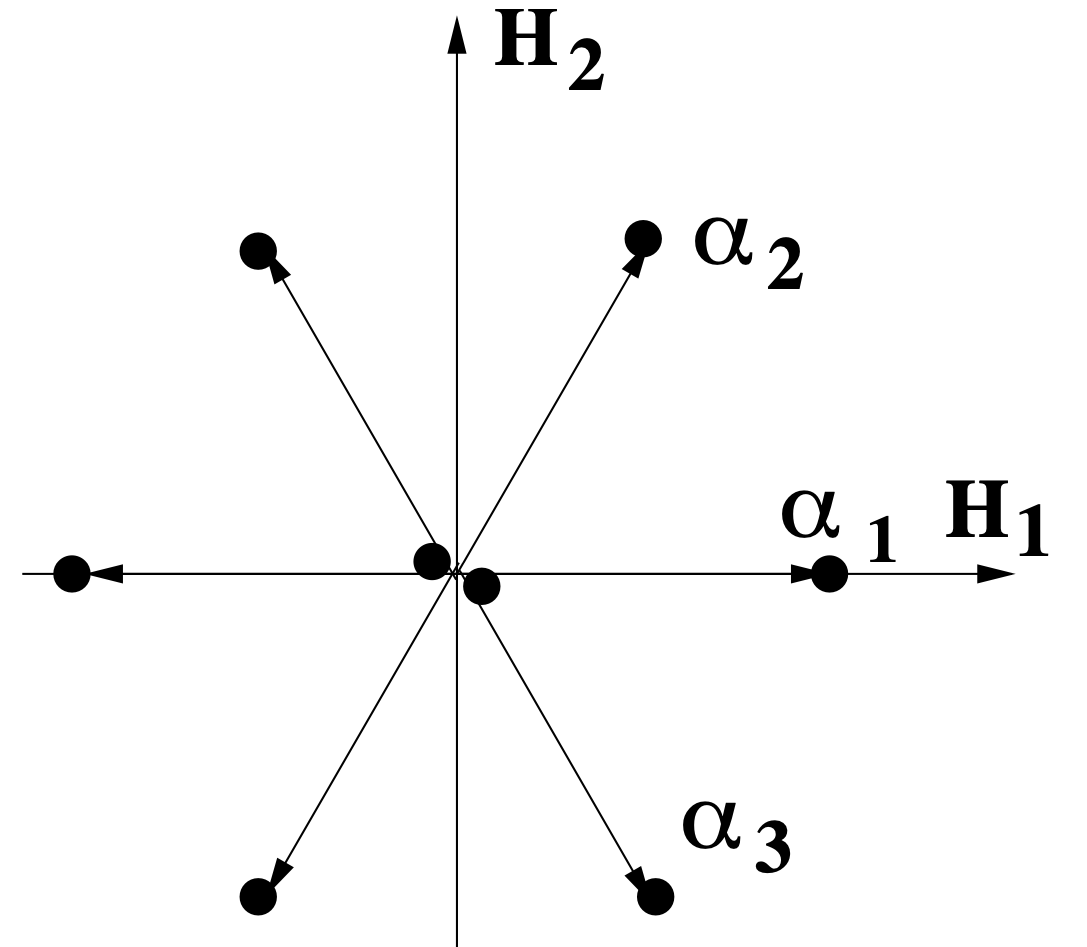
\includegraphics[width=0.3\textwidth]{figures/su3-root.png}
    \caption{The root system of the $SU(3)$ Lie algebra. The positive roots are $\alpha_1 = (1,0)$, $\alpha_2 = (1/2, 1/(2\sqrt{3}))$, $\alpha_3 = (1/2, -1/(2\sqrt{3}))$. The two roots at $(0,0)$ correspond to the Cartan generators.}
    \label{fig:su3-root-diagram}
\end{figure}

We can observe that the rank is $2$, which means the Cartan subalgebra is spanned by two generators $H_1$ and $H_2$, which are mutually commuting. The remaining $8$ generators are labelled by $E_\alpha$ and $E_{-\alpha}$, for $\alpha = (1,0), (1/2, 1/(2\sqrt{3})), (1/2, -1/(2\sqrt{3}))$, with commutation relations
\begin{equation}
    \comm{H_i}{E_{\pm \alpha}} = \pm \alpha_i E_{\pm \alpha} .
\end{equation}
The $SU(2)$ subalgebras for different $\alpha$ correspond, graphically, to the lines along which the roots reproduce the root diagram of $SU(2)$, in figure~\ref{fig:su2-root-diagram}.

Further, instead of writing explicit matrices providing a particular representation of the $SU(3)$ algebra, we can instead provide the weight diagram of the corresponding representation. As an example, the fundamental representation has complex dimension $3$, and the generators are represented by $8$ \emph{Gell-Mann matrices}. Upon exponentiation, the group elements are represented by $3 \times 3$ unitary matrices.

\begin{figure}
    \centering
    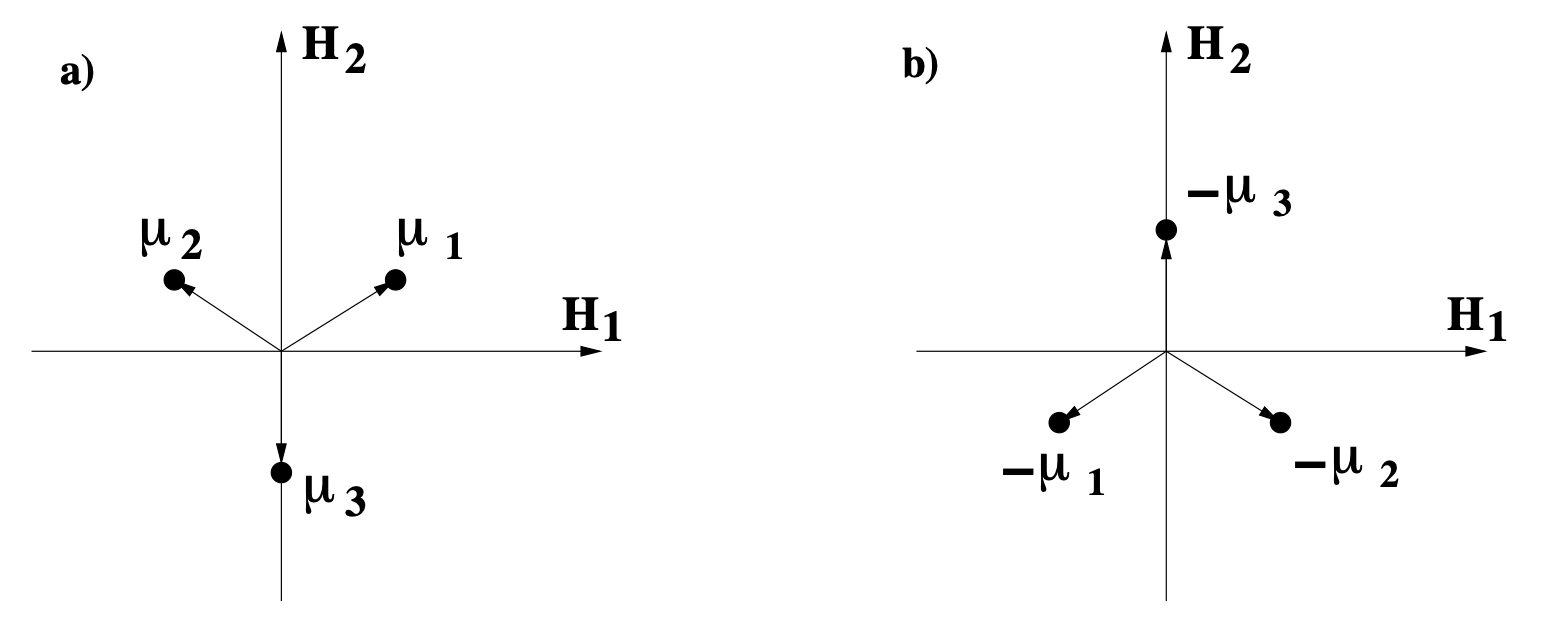
\includegraphics[width=0.7\textwidth]{figures/su3-weights.png}
    \caption{The weight diagram for the fundamental (a) and the antifundamental (b) representations of $SU(3)$. In particular $\mu_1 = (1/2, 1/(2\sqrt{3}))$, $\mu_2 = (-1/2, 1/(2\sqrt{3}))$ and $\mu_3 = (0, -1/\sqrt{3})$.}
    \label{fig:weight-su3-fund}
\end{figure}

This representation can be equivalently descibed by the weights in figure~\ref{fig:weight-su3-fund}. The action of the Cartans on the states $\ket{\mu = (\pm 1/2, 1/(2\sqrt{3})), (0,-1/\sqrt{3})}$ is
\begin{equation}
    H_i \ket{\mu} = \mu_i \ket{\mu} ,
\end{equation}
while the action of non-zero root generators $E_\alpha$ is
\begin{equation}
    E_\alpha \ket{\mu} = N_{\mu,\alpha}\ket{\mu + \alpha} .
\end{equation}

Notice that the states form representations under the $SU(2)$ subalgebras of the non-zero roots. That is, weights along lines parallel to the root diagram of the corresponding $SU(2)$ subgroup differ by the corresponding root.

The construction of irreducible representations is as follows. The highest weight is $\ket{\mu_1} = \ket{(1/2, 1/(2\sqrt{3}))}$, and is annihilated by the positive roots $\alpha_1 = (1,0)$, $\alpha_2 = (1/2, 1/(2\sqrt{3}))$ and $\alpha_3 = (1/2, -1/(2\sqrt{3}))$. The remaining states are obtained as
\begin{equation}
\begin{aligned}
    E_{-\alpha_1} \ket{(1/2,1/(2\sqrt{3}))} &\simeq \ket{(-1/2,1/(2\sqrt{3}))} ,\\
    E_{-\alpha_3} \ket{(1/2, 1/(2\sqrt{3}))} & \simeq \ket{0, -1/\sqrt{3}} .
\end{aligned}
\end{equation}

The conjugate representation, the antifundamental, which is obtained by minus the transposed Gell-Mann matrices, has weights opposite to those of the fundamental. Namely, conjugation of the representation flips the charges of objects. The weights are shown in figure~\ref{fig:weight-su3-fund}.

%*********************** DYNKIN DIAGRAMS *************************
\section{Dynkin Diagrams}
\paragraph{Angle of Roots}
Recall the master formula~\eqref{eq:master-formula}. It gives us a constraint of the weights, by requiring that $\ket{\mu + k\alpha}$ is a representation of $SU(2)_\alpha$, where $k \in \N$. We can apply it to the adjoint representation, where the weights $\mu$ are roots. Then, we can require that the states $\ket{\beta + k \alpha}$ form a representation of $SU(2)_\alpha$, and that the states $\ket{\alpha + k \beta}$ form a representation of $SU(2)_\beta$, getting
\begin{equation}
    \frac{\alpha \cdot \beta}{\abs{\alpha}^2} = - \frac{1}{2} m , \quad \frac{\beta \cdot \alpha}{\abs{\beta}^2} = - \frac{1}{2} m', \quad m, m' \in \Z.
\end{equation}

Then, we obtain a constraint on the relative angle of the roots, namely
\begin{equation}
    \cos^2 \theta_{\alpha\beta} \equiv \frac{(\alpha\cdot\beta)^2}{\abs{\alpha}^2\abs{\beta}^2} = \frac{mm'}{4}.
\end{equation}
The angle is constraint to be $0,30,45,60,90,120,135,150,\textup{or} \, 180$ degrees.

\paragraph{Simple Roots}
We define a \emph{simple root} as a positive root which cannot be written as a sum of positive roots with positive coefficients. One can show that the set of simple roots of an algebra is linearly independent and form a basis of the root space.

Further, one can see that the angle of simple roots is more constraint. To show this, let's first notice that if $\alpha$ and $\beta$ are simple roots, then $\alpha - \beta$ is \emph{not} a root. Indeed, if it were a root, it would be either positive or negative. If it is positive, then $\alpha = \beta + (\alpha - \beta)$ contradicts the fact that $\alpha$ is simple, while if it is negative, then $\beta = \alpha - (\alpha - \beta)$ contradicts that $\beta$ is simple.

Going in the adjoint representation, $E_{-\alpha}$ must annihilate $\ket{E_\beta}$, which makes it the lower weight state $\ket{-j}$ for the subalgebra $SU(2)_\beta$. Otherwise, $E_{-\alpha} \ket{E_\beta} \propto \ket{E_{\beta - \alpha}}$, but this is not possible since $\beta - \alpha$ is not a root. Then, with a similar argument used to derive the master formula~\eqref{eq:master-formula}, and inverting the roles of $\alpha$ and $\beta$, we get
\begin{equation}
    2 \frac{\alpha \cdot \beta}{\abs{\alpha}^2} = - p, \quad 2 \frac{\beta \cdot \alpha}{\abs{\beta}^2} = -p'  \quad p,p' \in \N .
\end{equation}

Therefore,
\begin{equation}\label{appeq:cosine}
    \cos \theta_{\alpha\beta} = -\frac{1}{2} \sqrt{pp'},
\end{equation}
which constraints the angles between simple roots to be $90,120,135,\text{or}\,150$ degrees.

\paragraph{Cartan Classification}
The \emph{relative lengths} and \emph{relative angles} are invariants of the set of simple roots. Using that simple roots provides a basis of the root space, one can recover the complete system of roots using the invariants. Then, the problem of classifying the Lie algrebras is reduced to the problem of classifying sets of $r$ linearly independent vectors in $r$-dimensional space with non-positive integer values of $2\frac{\alpha \cdot \beta}{\abs{\alpha}^2}$.

Before moving on, let's notice that if we have two systems of simple roots, of dimensions $r_1$ and $r_2$, we can combine them to form a $(r_1 + r_2)$-dimensional simple root system, by joining orthogonally the two initial systems. We're interested in root systems which can't be split into orthogonal subsystems. This is related to the concept of invariant subalgebras.

Given an algebra $A$, an \emph{invariant subalgebra} is a subalgebra such that the commutator of any element of $B$ with any element of $A$ is still in $A$. Upon exponentiation, Lie algebras with invariant subalgebras lead to \emph{non-simple} groups, which are groups which split as product of groups, like $G = G_1 \times G_2$. A Lie algebra without invariant subalgebras are called \emph{simple Lie algebra}.

So, in principle, we're interested in classifying simple groups and simple Lie algebras, since the others can be derived from them. One can further show that Lie algebras with invariant subalgebras manifest as root systems which split into two othogonal subsystems. Hence, we're interested in classifying \emph{simple root systems}, which don't have such subsystems. Any other system can be obtained by adjunction. 

\begin{figure}
    \centering
    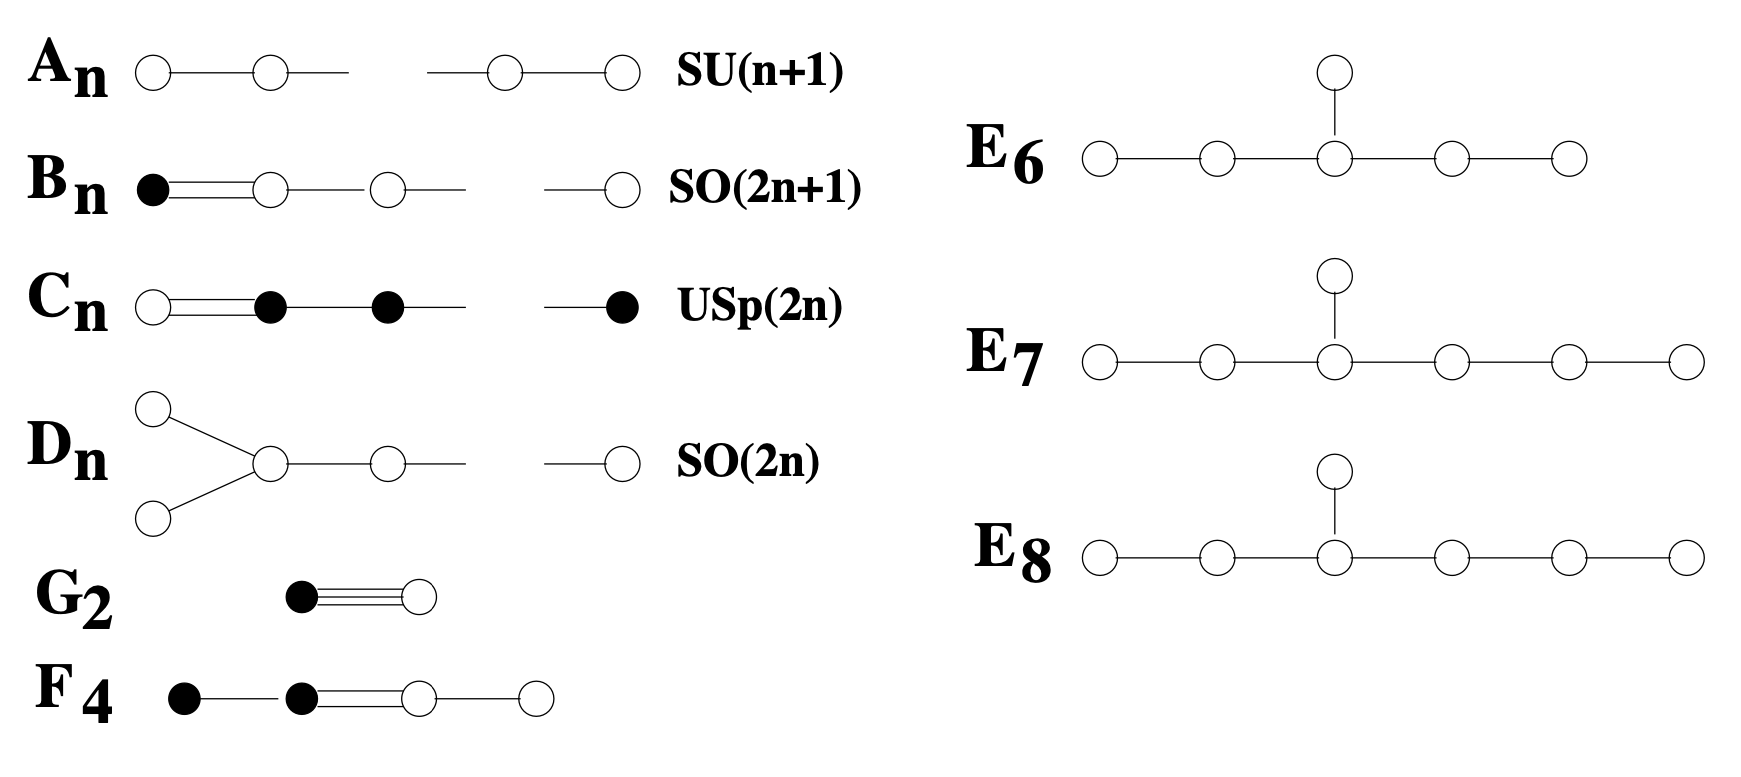
\includegraphics[width=0.75\textwidth]{figures/dynkin.png}
    \caption{Dynkin diagrams for simple Lie algebras. There are four infinite series (labelled by a positive integer $r$, giving the number of nodes), and some exceptional algebras. Notice that for small rank some algebras are isomorphic and have the same Dynking diagram (e.g., $A_3 = D_3$, namely $SU(4) \simeq SO(6)$). The groups arising from the $A$, $B$, $C$, and $D$ series were known in classical mathematics before Cartan and are known as classical Lie groups, they are listed to the right of the corresponding diagram.}
    \label{fig:dynkin}
\end{figure}

The problem of classifying simple root systems of this kind has been solved. The result, called the \emph{Cartan classification}, can be recast in giving the relative lengths and angles between the simple roots. This is conveniently represented in the \emph{Dynkin diagram}. The classification of Dynkin diagrams for simple Lie algebras is given in figure~\ref{fig:dynkin}. 

The rules to obtain the simple root system from the diagram are as follows:
\begin{itemize}
    \item each node corresponds to a simple root. Hence, the number of nodes is the rank of the Lie algebra/group;
    \item the number of lines joining two nodes gives us the angle between the two simple roots: no line means $90$°, one line means $120$°, two lines means $135$°, three lines means $150$°;
    \item dark nodes correspond to shorter roots. The relative lengths can be found from eq.~\eqref{appeq:cosine}.
\end{itemize}

Clearly, Dynking diagrams corresponding to non-simple algebras are obtained by adjoining in a disconnected way Dynkin diagrams for simple algebras, so that we adjoin orthogonally the two subsystems of simple roots.

%*********************** SU(K) GROUP *************************
\section{The Group \texorpdfstring{$SU(k)$}{SU(k)}}
\paragraph{Roots}
Although $SU(k)$ (or its algebra $A_{k-1})$ has rank $k-1$, it is convenient and easier to describe its roots as $k$-dimensional vectors, which lie on an $(k-1)$-plane. Besides the $k-1$ zero roots associated to the Cartan generators, the non-zero roots are given by the $k$-dimensional vectors  
\begin{equation}
    (\underline{+,-,0,\dots,0}),
\end{equation}
where $+,-$ denote $+1, -1$, and where underlining means permutation, namely the $+$ and $-$ can be located in any (non-coincident) positions. Note that all roots satisfy one relation $\sum_{i=1}^n v_i = 0$, so they live in a $(k-1)$-plane $\Pi$ in $\R^n$. There are a total of $k^2-1$ roots, which is the number of generators of $SU(k)$.

Fixing a basis within the $(k-1)$-plane it is straightforward to read out the roots as $(k-1)$-dimensional vectors. The picture of the root system of $SU(3)$ in this language is given in figure~\ref{fig:su3-root-system}.

\begin{figure}
    \centering
    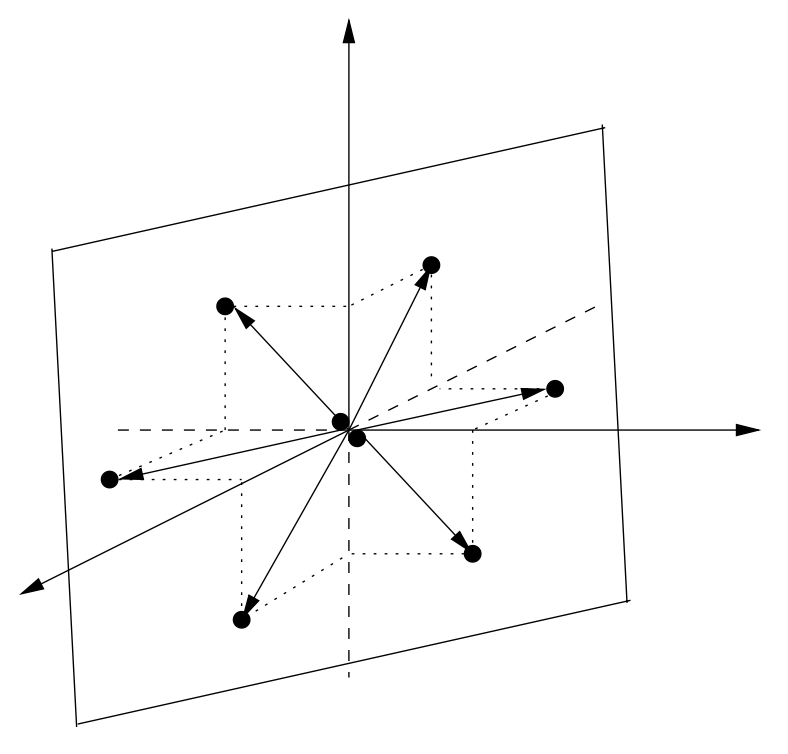
\includegraphics[width=0.4\textwidth]{figures/su3-root-system.png}
    \caption{The root system of $SU(3)$ described as a set of vectors lying in a $2$-plane in $3$-dimensional space.}
    \label{fig:su3-root-system}
\end{figure}

The extra direction in the diagram can be regarded as associated to the extra $U(1)$ generator in $U(k) = SU(k) \times U(1)$. Hence, $SU(k)$ weight diagrams embedded in $(k-1)$-planes parallel to $\Pi$ but not passing through the origin are associated to states which, in addition to being in a representation of $SU(k)$, also carry some charge under the additional $U(1)$.

\paragraph{Weights}
A familiar representation is the fundamental representation. The corresponding weights, given as $k$-dimensional vectors but inside the $(k-1)$-plane $\Pi$ are,
\begin{equation}\label{appeq:fund-weights}
    \frac{1}{n} (\underline{n-1, -1, \dots, -1}) .
\end{equation}
Notice that weights differ by roots, so application of generators associated to non-zero roots relate states with different weights (or give zero if they take us out of the representation).
In situations where the gauge group is $U(k)$, so there is an additional $U(1)$ generator, the fundamentals of $SU(k)$ may carry some charge, so the weights satisfy the relation $\sum_{i=1}^n v_i = q$, for some non-zero constant $q$ giving (up to normalization) the charge under the additional $U(1)$. Very often one finds fundamentals from weights of the form
\begin{equation}\label{appeq:fund1}
    (\underline{+,0,\dots,0}),
\end{equation}
or
\begin{equation}\label{appeq:fund2}
    \frac{1}{2} (\underline{+,-,dots,-}).
\end{equation}

Notice that the weights~\eqref{appeq:fund-weights} can be written as
\begin{equation}
    (\underline{+,0,\dots,0}) - (1/n, \dots, -1/n),
\end{equation}
where the second term removes the piece corresponding to the additional $U(1)$ charge. By abuse of language, we will often use things expressions like~\eqref{appeq:fund1} or~\eqref{appeq:fund2} to denote the fundamental even in situations where there is no additional $U(1)$, removing implicitly the piece corresponding to this charge.

The weights for the antifundamental representation are the opposite to those for the fundamental, namely
\begin{equation}
    (\underline{-,0,\dots,0}).
\end{equation}
By this, we mean
\begin{equation}
    \frac{1}{n} (\underline{-(n-1),1,\dots,1}),
\end{equation}
or any other shifted version, with the understanding that the additional $U(1)$ charge should be removed.

Other representations can be obtained by taking tensor products of the
fundamental, and the corresponding weights are obtained by adding the weights of the fundamental representation.

For instance, the two-index antisymmetric representation has $k(k-1)/2$ weights
\begin{equation}
    (\underline{+,+,0,\dots,0}),
\end{equation}
while the two-index symmetric representation has $k(k+ 1)/2$ weights
\begin{equation}
    (\underline{+,+,0,\dots,0}), \quad (\underline{\pm 2, 0, \dots, 0}).
\end{equation}
They are obtained by adding two times weights of the fundamental representation in a way consistent with antisymmetry or symmetry of the representation.

It is straightforward to derive familiar facts like the equivalence of the antifundamental representation and the $(k-1)$-index antisymmetric representation. They have the same weights.


%*********************** SO(2r) GROUP *************************
\section{The Group \texorpdfstring{$SO(2r)$}{SO(2r)}}
\paragraph{Roots}
Besides the $n$ zero roots, the non-zero roots for the $D_r$ Lie algebra are given by the $r$-dimensional vectors
\begin{equation}
    (\underline{\pm,\pm,0,\dots,0}),
\end{equation}
meaning that the $+$ and $-$ can be choses arbitrarily in any non-coincident position. The total number of roots is $2r(2r-1)/2$.

\begin{figure}
    \centering
    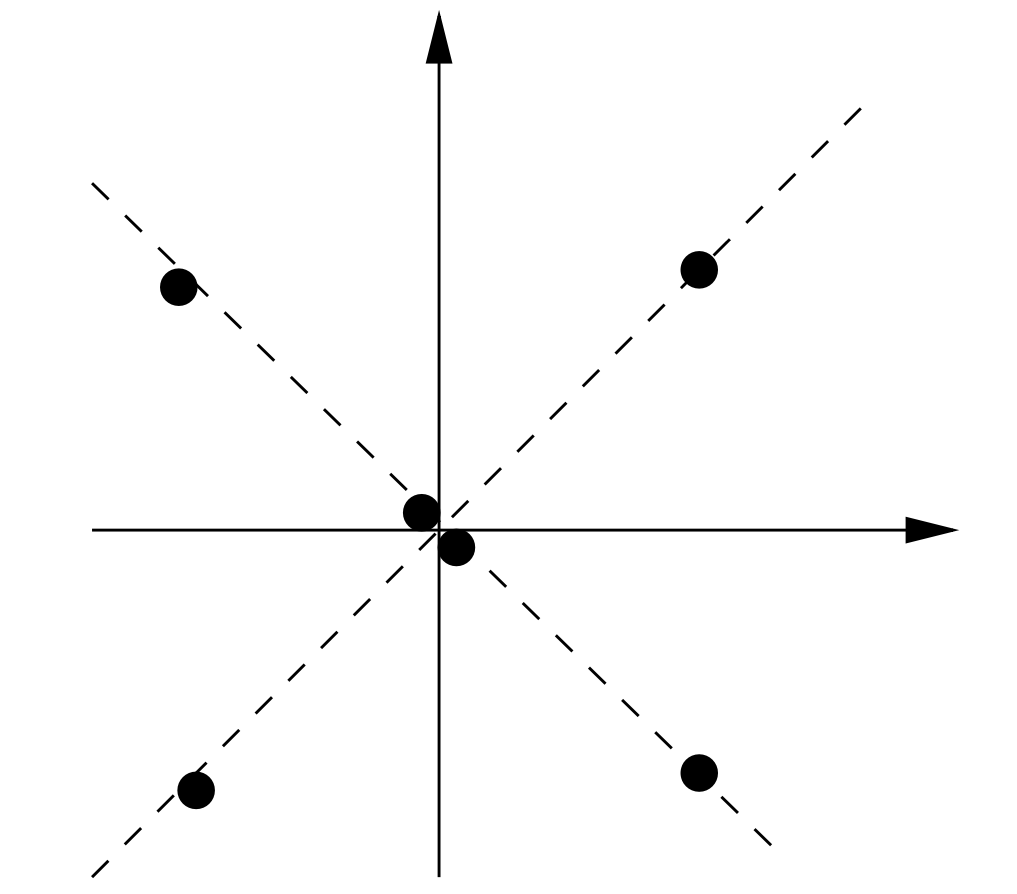
\includegraphics[width=0.35\textwidth]{figures/so4-root-system.png}
    \caption{ Root diagram for $SO(4)$. In fact, it splits as two orthogonal $SU(2)$ root systems.}
    \label{fig:so4-root-system}
\end{figure}

The root system of $SO(4)$ is shown in figure~\ref{fig:so4-root-system}. The fact that there are
two subsets of orthogonal roots means that there are invariant subalgebras. In fact, $SO(4) \simeq SU(2) \times SU(2)'$, with non-zero roots of the latter being given by
\begin{equation}
    SU(2): (+,+),\,(-,-), \quad SU(2)': (+-),\,(-+) .
\end{equation}
Notice also that the Dynkin diagram for $D_2$ are two disconnected nodes, so is the same as two $A_1$ Dynkin diagrams.

It is important to notice that the root system of $SO(2r)$ contains the roots of $SU(r)$, so by exponentiation the group $SO(2r)$ contains a subgroup $SU(r)$.

\paragraph{Weights}
An important representation is the \emph{vector representation}, which is $2r$-dimensional and has weights
\begin{equation}
    (\underline{\pm,0,\dots,0}).
\end{equation}
Notice that it is a real representation, since its conjugate has opposite weights, but the representation (as a whole) is invariant under such change.

When the group is regarded as the group of rotational isometries of a $2r$-dimensional euclidean space, the vector representation in which vectors of this space transform.

More representations can be obtained by taking tensor products of the vector representation. These are the representations under which tensors in the euclidean space transform under rotations.

There are some additional representations which cannot be obtained from tensor products of the vector representation. These are the spinor representations. For $D_r$ there are two inequivalent irreducible spinor representations, both with dimension $2^{r-1}$, and weights
\begin{equation}
\begin{aligned}
    \textup{spinor}: \quad  &\left(\pm\frac{1}{2}, \dots, \pm \frac{1}{2}\right), \quad \textup{$\#-=$even}, \\
    \textup{spinor'}: \quad &\left(\pm\frac{1}{2}, \dots, \pm \frac{1}{2}\right), \quad \textup{$\#-=$odd}.
\end{aligned}
\end{equation}
These spinor representations are said to have different chirality

%*********************** CLIFFORD ALGEBRA *************************
\section{Spinor Representations and Clifford Algebra}
There is a canonical and very useful way to describe the spinor representations of $SO(2r)$, related to representations of Clifford algebras.

Consider the algebra of objects $\Gamma^i$, $i = 1, \dots, 2r$, satisfying
\begin{equation}\label{appeq:clifford}
    \{\Gamma^i, \Gamma^j\} = 2 \delta_{ij}.
\end{equation}
It is called a Clifford algebra.

The important point is that this algebra is invariant under the group of transformations
\begin{equation}
    \Gamma'^i = R^i_j \Gamma^j,
\end{equation}
where $R$ is a $2r\times2r$ orthogonal matrix. This group is precisely $SO(2r)$, and we have found it acting on the set of $\Gamma^i$ in the fundamental representation.

The fact that the Clifford algebra~\eqref{appeq:clifford} has an $SO(2r)$ invariance menas that any representation of the Clifford algebra must also form a representation of $SO(2r)$. In fact, given a hermitian matrix representation for the $\Gamma^i$, the hermitian matrices $J^{ij} = -\frac{i}{4}\comm{\Gamma^i}{\Gamma^j}$ can be seen to form a (possibly reducible) hermitian matrix representation of the $SO(2r)$ algebra, which is
\begin{equation}
    \comm{J^{ij}}{J^{kl}} = i \left( \delta^{ik} J^{jl} + \delta^{jl} J^{ik} - \delta^{il} J^{jlk} - \delta^{jk} J^{il} \right)
\end{equation}

So our purpose is to build a representation of the Clifford algebra, and the resulting representations of $SO(2r)$. The standard technique to build a representation of the Clifford algebra is to form linear combinations of the $\Gamma^i$ which can act as raising and lowering operators. We define
\begin{equation}
    A_a = \frac{1}{\sqrt{2}} (\Gamma_{2a}+i \Gamma_{2a-1}), \quad A^\dagger_a = \frac{1}{\sqrt{2}} (\Gamma_{2a}-i \Gamma_{2a-1}), \quad  a = 1, \dots, r .
\end{equation}
They satisfy the relations
\begin{equation}
    \{ A^\dagger_a, A^\dagger_b \} = \{ A_a, A_b \} = 0, \quad \{A^\dagger_a, A_b\} = \delta_{ab} .
\end{equation}
So they behave as fermionic oscillator ladder operators. Notice that in this language only an $SU(r)$ invariance is manifest, with the $A^\dagger_a$, $A_a$ transforming in the fundamental and antifundamental representations, respectively.

To build a representation of the Clifford algebra, we introduce a “ground-state” for the harmonic oscillator
\begin{equation}
    A_a \ket{0} = 0.
\end{equation}
The representation is built by applying raising operators to this “ground-state” in all possible inequivalent ways. We have
\begin{equation}\label{appeq:states-harmonic-osc}
\begin{aligned}
    \textup{states} \quad &\textup{numbers} \\
    \ket{0} \quad &1  \\
    A^\dagger_a\ket{0} \quad &r \\
    A^\dagger_a A^\dagger_b \ket{0} \quad &r(r-1)/2 \\
    \dots \quad &\dots \\
    A^\dagger_{a_1} \dots A^\dagger_{a_k} \ket{0} \quad &\binom{r}{k} \\
    \dots \quad &\dots \\
    A^\dagger_1 \dots A^\dagger_r \ket{0} \quad &1
\end{aligned}
\end{equation}
The bunch of $\binom{r}{k}$ states arising from applying $k$ operators to the ground-state clearly forms a $k$-index completely antisymmetric tensor representation of the $SU(r)$ invariance group.

The total number of states is $2^r$. Constructing the Lorentz generators, it is possible to check that the weights are of the form
\begin{equation}
    \left( \pm \frac{1}{2}, \dots, \frac{1}{2} \right).
\end{equation}
Moreover, it is easy to realize that the weights among the above with has $k +1/2$'s correspond to the weights of a $k$-index completely antisymmetric tensor representation of $SU(r)$, in agreement with our above statement.

The above weights therefore define a representation of the $SO(2r)$ group (although only $SU(r)$ invariance was manifest in intermediate steps). Now, this representation is reducible. Recalling that the $SO(2r)$ generators are constructed with products of two $\Gamma^i$'s, it is clear that they are unable to relate states~\eqref{appeq:states-harmonic-osc} with even number of $\Gamma$'s to states with odd number of $\Gamma$'s. 

More formally, one can introduce the chirality operator $\Gamma = \Gamma^1 \dots \Gamma^{2r}$ which commutes with all $SO(2r)$ generators (and anticommutes with the $\Gamma^i$), and can be used to distinguish the two subsets of states.

This means that the $2^r$-dimensional representation is reducible into two $2^{r-1}$-dimensional irreducible representations.

\bibliography{bibliography.bib}

\end{document}
